\documentclass[lang=cn,newtx,10pt,scheme=chinese]{elegantbook}

\title{《算法导论第四版》学习笔记}
\author{左元}

\setcounter{tocdepth}{3}

\cover{算法导论第四版插图/封面.pdf}

% 本文档命令
\usepackage{array}
\newcommand{\ccr}[1]{\makecell{{\color{#1}\rule{1cm}{1cm}}}}

% 修改标题页的橙色带
\definecolor{customcolor}{RGB}{32,178,170}
\colorlet{coverlinecolor}{customcolor}
\usepackage{cprotect}

\begin{document}

\maketitle
\frontmatter

\tableofcontents

\mainmatter

\part{基础知识}

\chapter*{简介}

当你设计和分析算法时,你需要能够描述算法的运行方式以及如何设计算法。你还需要一些数学工具来证明你的算法是正确且高效的。这部分内容将帮助你入门。本书的后续部分将在此基础上展开。

第1章提供了算法及其在现代计算系统中的位置的概述。本章定义了算法的概念并列举了一些例子。它还提出了将算法视为一种技术的观点,与高速的硬件、图形用户界面(GUI)、面向对象系统和网络等技术并列。

在第2章中,我们首次见到了解决排序$n$个数字序列问题的算法。它们以伪代码形式编写,虽然不能直接转换为任何传统的编程语言,但足够清晰地传达了算法的结构,以便你能够在自己选择的编程语言中实现它。我们研究的排序算法包括插入排序(使用增量方法)和归并排序(使用递归技术,称为“分而治之”)。虽然每个算法所需的时间随$n$的值增加而增加,但增长的速率在这两个算法之间有所不同。我们在第2章中确定了这些运行时间,并开发了一个有用的“渐近”符号来表示它们。

第3章对渐近符号进行了精确定义。我们将使用渐近符号来界定函数的增长范围,最常见的情况是描述算法运行时间的函数,上下界都包括在内。该章节首先非正式地定义了最常用的渐近符号,并给出了如何应用它们的示例。然后,它正式地定义了五种渐近符号,并介绍了将它们组合使用的约定。第3章的其余部分主要是数学符号的展示,更多地是为了确保你使用的符号与本书一致,而不是教授你新的数学概念。

第4章进一步探讨了第2章中介绍的分治策略。它提供了两个额外的示例,展示了用于相乘方阵的分治算法,其中包括令人惊讶的Strassen算法。第4章介绍了解决递归关系的方法,这对描述递归算法的运行时间很有用。在代入法中,你猜测一个答案并证明它的正确性。递归树提供了一种生成猜测的方法。第4章还介绍了强大的“主方法”技术,你通常可以使用它来解决由分而治之算法引起的递归关系。虽然该章节提供了主定理所依赖的基础定理的证明,但你可以自由地使用主方法,而不必深入研究证明。第4章以一些高级主题结束。

第5章介绍了概率分析和随机算法。通常,你使用概率分析来确定算法的运行时间,在这种情况下,由于固有的概率分布的存在,相同大小的不同输入可能具有不同的运行时间。在某些情况下,你可能会假设输入符合已知的概率分布,以便对所有可能的输入求平均运行时间。在其他情况下,概率分布不是来自输入,而是来自算法执行过程中所做的随机选择。一个算法的行为不仅由其输入决定,还由随机数生成器产生的值决定,这就是随机算法。你可以使用随机算法来对输入强制施加概率分布,从而确保没有特定的输入会导致性能下降,甚至用于限制允许产生错误结果的算法的错误率。

附录A-D包含其他数学材料,在阅读本书时对你会有帮助。你可能在阅读本书之前已经看过附录章节中的大部分内容(尽管我们使用的特定定义和符号约定在某些情况下可能与你之前看到的有所不同),所以你应该将附录视为参考资料。另一方面,你可能尚未看到第一部分的大部分材料。第一部分的所有章节和附录都以教程风格编写。

\chapter{算法在计算中的作用}

什么是算法?为什么研究算法是值得的?相对于计算机中使用的其他技术,算法的作用是什么?本章将回答这些问题。

\section{算法}

非正式地说,算法是一种明确定义的计算过程,它以某些值或一组值作为输入,并在有限时间内产生某些值或一组值作为输出。因此,算法是一系列计算步骤,将输入转化为输出。

你也可以将算法视为解决明确定义的计算问题的工具。问题的陈述以一般性的方式指定了问题实例的所需输入/输出关系,通常是任意大的问题实例。算法描述了一种特定的计算过程,以实现所有问题实例的输入/输出关系。

举个例子,假设你需要将一组数字按照单调递增的顺序进行排序。这个问题在实践中经常出现,并为引入许多标准的设计技术和分析工具提供了丰富的素材。以下是我们如何正式定义排序问题:

\textbf{输入}:$n$ 个数的一个序列 $\langle a_1, a_2, ..., a_n\rangle$。

\textbf{输出}:输入序列的一个排列(排序之后的) $\langle{a'_1,a'_2,...,a'_n}\rangle$,满足$\langle{a'_1\le a'_2\le \cdots\le a'_n}\rangle$。

因此,给定输入序列$\langle{31,41,59,26,41,58}\rangle$,一个正确的排序算法将输出序列 $\langle{26,31,41,41,58,59}\rangle$。这样的输入序列被称为排序问题的一个实例。一般来说,问题的一个实例包括计算问题解所需的输入(满足问题陈述中规定的约束条件)。

由于许多程序将其作为中间步骤使用,排序是计算机科学中的一项基本操作。因此,你可以选择使用许多优秀的排序算法。哪种算法对于给定的应用程序最佳取决于多个因素,包括待排序项的数量,项的部分排序程度,对项值可能存在的限制,计算机的体系结构以及要使用的存储设备类型:主内存、磁盘,甚至是过时的磁带。

对于一个计算问题的算法,如果对于每个作为输入提供的问题实例,它能在有限的时间内停止计算,并输出问题实例的正确解,那么这个算法是正确的。一个正确的算法解决了给定的计算问题。而一个不正确的算法可能在某些输入实例上根本无法停止计算,或者在停止时给出错误的答案。与你可能期望的相反,如果能够控制错误率,不正确的算法有时也可能是有用的。当我们学习用于查找大素数的算法时,我们将在第31章中看到一个具有可控错误率的算法的例子。然而,通常情况下,我们只关注正确的算法。

算法可以用英语、计算机程序甚至硬件设计来进行规定。唯一的要求是规定必须提供对应计算过程的精确描述。

\textbf{算法解决哪种问题}

排序远非唯一一个已经开发出算法的计算问题。(当你看到本书的厚度时,你可能已经怀疑到这一点。)算法的实际应用无处不在,包括以下示例:

\begin{itemize}
    \item 人类基因组计划在实现以下目标方面取得了巨大进展:鉴定人类DNA中大约3万个基因,确定构成人类DNA的大约30亿个化学碱基对的序列,将这些信息存储在数据库中,并开发用于数据分析的工具。每个步骤都需要复杂的算法。虽然这些问题的解决方案超出了本书的范围,但许多解决这些生物学问题的方法使用了本书中介绍的思想,使科学家能够在有效利用资源的同时完成任务。动态规划(如第14章所述)是解决其中几个生物学问题的重要技术,特别是涉及确定DNA序列之间相似性的问题。这样做可以节省时间(包括人力和机器时间)和金钱,因为实验技术可以提取更多的信息。
    \item 互联网使全球人民能够快速访问和检索大量信息。借助巧妙的算法,互联网上的网站能够管理和操作这些大量的数据。一些必须使用算法的问题的示例包括找到数据传输的良好路径(解决此类问题的技术出现在第22章),以及使用搜索引擎快速找到包含特定信息的网页(相关技术在第11章和第32章)。
    \item 电子商务使得商品和服务能够在电子环境下进行协商和交换,并且它依赖于个人信息的隐私,例如信用卡号码、密码和银行对账单。电子商务中使用的核心技术包括公钥加密和数字签名(在第31章中介绍),这些技术基于数值算法和数论。
    \item 制造业和其他商业企业经常需要以最有利的方式分配稀缺资源。石油公司可能希望知道在哪里安置油井以最大化预期利润。政治候选人可能希望确定在哪里花钱购买竞选广告,以最大化赢得选举的机会。航空公司可能希望以最低成本的方式为航班分配机组,确保每个航班得到覆盖,并满足政府对机组排班的规定。互联网服务提供商可能希望确定在哪里投放额外资源,以更有效地为其客户提供服务。所有这些都是可以通过将它们建模为线性规划问题来解决的例子,这是第29章讨论的内容。
\end{itemize}

尽管这些例子的一些细节超出了本书的范围,但我们确实介绍了适用于这些问题和问题领域的基本技术。我们还展示了如何解决许多具体问题,包括以下问题:

\begin{itemize}
    \item 你手上有一张道路地图,上面标记了相邻交叉口之间的距离,你希望确定从一个交叉口到另一个交叉口的最短路径。即使不允许路径相交,可能的路径数量也可能非常大。你如何选择所有可能路径中最短的一条呢?你可以首先将道路地图(它本身就是实际道路的模型)建模为一个图(我们将在第六部分和附录B中介绍)。在这个图中,你希望找到从一个顶点到另一个顶点的最短路径。第22章展示了如何高效解决这个问题。
    \item 给定一个以零件库形式表示的机械设计,其中每个零件可能包含其他零件的实例,按顺序列出零件,使得每个零件都出现在使用它的任何零件之前。如果设计包含$n$个零件,则存在$n!$种可能的顺序,其中$n!$表示阶乘函数。由于阶乘函数的增长速度甚至超过指数函数,你不可能可行地生成每个可能的顺序,然后验证在该顺序中,每个零件都出现在使用它的零件之前(除非只有几个零件)。这个问题是拓扑排序的一个实例,第20章展示了如何高效解决这个问题。
    \item 医生需要确定一张图像是否代表了一个恶性肿瘤或良性肿瘤。医生有很多其他肿瘤的图像可用,其中一些已知是恶性的,一些已知是良性的。恶性肿瘤很可能与其他恶性肿瘤更相似,而良性肿瘤更可能与其他良性肿瘤相似。通过使用聚类算法,如第33章所示,医生可以确定哪种结果更有可能。
    \item 你需要对一个包含文本的大文件进行压缩,以便占用更少的空间。有许多已知的方法可以实现这一目的,包括``LZW压缩算法'',它寻找重复的字符序列。第15章研究了一种不同的方法,即``Huffman编码'',它通过不同长度的位序列对字符进行编码,其中出现频率更高的字符使用较短的位序列进行编码。
\end{itemize}

这些列表远非详尽无遗(你可能从本书的厚度中推测出来了),但它们展示了许多有趣的算法问题所共有的两个特点:

\begin{enumerate}
    \item 它们有许多潜在的解决方案,其中绝大多数并不能解决手头的问题。在不显式地检查每个可能的解决方案的情况下,找到一个能够解决问题或是一个``最佳''解决方案,可能会带来相当大的挑战。
    \item 它们具有实际应用。在上述问题列表中,寻找最短路径提供了最简单的例子。运输公司,如货车或铁路公司,有着在道路或铁路网络中找到最短路径的经济利益,因为选择更短的路径可以降低劳动力和燃料成本。或者,互联网上的路由节点可能需要找到网络中的最短路径,以便快速路由一条消息。或者,一个想要从纽约开车到波士顿的人可能希望使用导航应用程序找到驾驶方向。
\end{enumerate}

并非每个由算法解决的问题都有一个容易确定的候选解集。例如,给定一组表示定期时间间隔取样的信号样本的数值,离散傅里叶变换将时间域转换为频率域。也就是说,它将信号近似为正弦波的加权和,产生不同频率的强度,这些频率的加和近似于取样信号。离散傅里叶变换除了是信号处理的核心之外,还在数据压缩和大多项式和整数乘法中具有应用。第30章介绍了这个问题的高效算法,即快速傅里叶变换(通常称为``FFT'')。该章还概述了一个硬件FFT电路的设计。

\textbf{数据结构}

这本书还介绍了几种数据结构。数据结构是一种存储和组织数据的方式,以便于访问和修改。选择适当的数据结构是算法设计的重要组成部分。没有一种单一的数据结构适用于所有目的,因此你应该了解其中几种数据结构的优势和限制。

\textbf{技术}

虽然你可以将本书作为算法的``菜谱''使用,但你可能会遇到一些问题,对于这些问题,你无法很容易地找到已发布的算法(例如,本书中的许多练习和问题)。本书将教你算法设计和分析的技巧,以便你能够独立开发算法,验证其正确性,并分析其效率。不同的章节涉及算法问题解决的不同方面。一些章节解决特定的问题,例如在第9章中找到中位数和顺序统计量,在第21章中计算最小生成树,在第24章中确定网络中的最大流。其他章节介绍了一些技术,例如在第2章和第4章中的分治法、第14章中的动态规划以及第16章中的摊还分析。

\textbf{难题}

本书的大部分内容都是关于高效算法的。我们通常衡量算法的效率是通过速度:一个算法产生结果需要多长时间?然而,有一些问题我们并没有找到在合理时间内运行的算法。第34章研究了这些问题中的一个有趣子集,被称为NP完全问题。

为什么NP完全问题很有趣?首先,尽管我们从未找到过NP完全问题的高效算法,但也没有人能够证明不存在高效算法。换句话说,没有人知道是否存在适用于NP完全问题的高效算法。其次,NP完全问题集合具有一个显著的特性,即如果其中任何一个问题存在高效算法,那么所有问题都存在高效算法。这种关系使得缺乏高效解决方案更加引人入胜。第三,几个NP完全问题与我们已知存在高效算法的问题相似但并不相同。计算机科学家对于问题陈述的微小变化如何导致已知最佳算法的效率发生巨大变化感到着迷。

你应该了解NP完全问题,因为它们在实际应用中出现得相当频繁。如果你需要为一个NP完全问题设计一个高效算法,你可能会花费很多时间进行无果的搜索。相反,如果你能证明该问题是NP完全问题,你可以把时间花在开发高效的近似算法上,也就是一种能够给出较好但不一定是最优解的算法。

举个具体的例子,考虑一个带有中央配送中心的送货公司。每天,公司会在中心配送中心装货,并将货物送到多个地址。在一天结束时,每辆卡车必须回到中心配送中心,以便准备下一天的装货。为了降低成本,公司希望选择一种送货顺序,使得每辆卡车行驶的总距离最小。这个问题就是著名的``旅行推销员问题'',它是一个NP完全问题。目前没有已知的高效算法。然而,在一定的假设条件下,我们知道有一些高效算法可以计算出接近最小总距离的解。第35章讨论了这种"近似算法"。

\textbf{可选计算模型}

多年来,我们可以指望处理器的时钟速度以稳定的速度增加。然而,物理限制对不断增长的时钟速度构成了根本性障碍:因为功率密度与时钟速度超线性增加,一旦时钟速度足够高,芯片就有熔化的风险。因此,为了每秒执行更多计算,芯片被设计成不仅包含一个处理"核心",而是几个处理核心。我们可以将这些多核计算机类比为在单个芯片上的几个顺序计算机。换句话说,它们是一种"并行计算机"。为了从多核计算机中获得最佳性能,我们需要设计考虑并行性的算法。第26章介绍了一种"任务并行"算法模型,它利用了多个处理核心。这个模型在理论和实践的角度都有优势,许多现代并行编程平台也采用了类似于这种并行模型的方法。

本书中的大部分示例假设在算法开始运行时所有输入数据都是可用的。算法设计的大部分工作也是基于这个假设进行的。然而,在许多重要的实际示例中,输入数据实际上是随时间到达的,而算法必须在不知道未来将到达的数据的情况下决定如何进行。在数据中心,作业不断到达和离开,调度算法必须决定何时何地运行作业,而不知道未来将会到达哪些作业。在互联网中,必须根据当前状态路由流量,而不知道未来流量将到达的位置。医院急诊室必须根据患者的病情进行分诊决策,而不知道未来其他患者何时到达以及他们需要哪些治疗。接收输入数据的算法并非一开始就具有所有输入,而是随着时间推移,这些算法被称为在线算法,第27章对其进行了研究。

\section{作为一种技术的算法}

如果计算机的速度是无限快的,计算机内存是免费的,你还有理由学习算法吗?答案是肯定的,即使没有其他原因,你仍然希望确保你的解决方法能够终止,并且以正确的答案终止。

如果计算机的速度是无限快的,任何正确的问题解决方法都可以。你可能希望你的实现符合良好的软件工程实践的要求(例如,你的实现应该设计良好并有文档说明),但你通常会选择最容易实现的方法。

当然,计算机可能很快,但它们并不是无限快的。计算时间是一种有限的资源,因此它非常宝贵。虽然有句谚语说“时间就是金钱”,但时间比金钱更宝贵:你可以在花费之后再获得金钱,但一旦时间花费了,就无法回收。内存可能不贵,但它既不是无限的,也不是免费的。你应该选择能够有效利用时间和空间资源的算法。

\textbf{效率}

不同的算法用于解决同一问题时,它们的效率常常有很大差异。这些差异可能比硬件和软件造成的差异更为显著。

以排序问题为例,第2章介绍了两种排序算法。第一种称为插入排序,它花费大约$c_1n^2$的时间来排序$n$个元素,其中$c_1$是一个与$n$无关的常数。也就是说,它的时间复杂度大约与$n^2$成正比。第二种归并排序,花费大约$c_2n\lg n$的时间,其中$\lg n$表示$log_2n$,$c_2$是另一个与$n$无关的常数。插入排序通常具有比归并排序更小的常数因子,因此$c_1 < c_2$。我们将看到,常数因子对运行时间的影响远远小于对输入规模$n$的依赖。我们将插入排序的运行时间写为$c_1n \cdot n$,归并排序的运行时间写为$c_2n \cdot \lg n$。然后我们可以看到,插入排序的运行时间中有一个$n$因子,而归并排序的运行时间中有一个$\lg n$因子,后者要小得多。例如,当$n$为1000时,$\lg n$大约为10,当$n$为1,000,000时,$\lg n$仅约为20。虽然对于小的输入规模,插入排序通常比归并排序运行更快,但一旦输入规模$n$足够大,归并排序的$\lg n$相对于$n$的优势将远远弥补常数因子的差异。无论$c_1$比$c_2$小多少,总有一个交叉点,在该点之后归并排序更快。

举一个具体的例子,我们比较一个运行插入排序的速度更快的计算机A与一个运行归并排序的速度较慢的计算机B。它们各自需要对一个包含1千万个数字的数组进行排序。(尽管1千万个数字可能看起来很多,但如果这些数字是8字节的整数,那么输入数据大约占用80兆字节的内存,即使是廉价的笔记本电脑的内存也能容纳多次。)假设计算机A每秒执行100亿条指令(比目前最快的任何顺序计算机都要快),而计算机B每秒只执行1000万条指令(比大多数当代计算机都要慢得多),因此计算机A的计算能力比计算机B高1000倍。为了使差距更加明显,假设世界上最聪明的程序员用机器语言为计算机A编写插入排序算法,所得到的代码需要$2n^2$条指令来对n个数字进行排序。进一步假设一个普通的程序员使用一个效率低下的编译器,使用高级语言实现了归并排序,所得到的代码需要$50n\lg n$条指令。对于排序1千万个数字,计算机A需要

$$
\frac{2\cdot (10^7)^2\text{条指令}}{10^{10}\text{条指令}/\text{秒}}
=
20,000\text{秒(大于5.5小时)}
$$

而计算机B需要

$$
\frac{50\cdot 10^7\lg 10^7\text{条指令}}{10^{10}\text{条指令}/\text{秒}}
=
1163\text{秒(少于20分钟)}
$$

通过使用一个增长速度较慢的算法,即使使用一个糟糕的编译器,计算机B的运行速度也比计算机A快了超过17倍!当对1亿个数字进行排序时,归并排序的优势更加明显:插入排序需要超过23天,而归并排序只需要不到4小时。虽然1亿可能看起来是一个很大的数字,但每半小时就有超过1亿次网络搜索,每分钟发送超过1亿封电子邮件,一些最小的星系(被称为超紧密矮星系)包含大约1亿颗恒星。一般来说,随着问题规模的增加,归并排序的相对优势也会增加。

\textbf{算法和其它技术}

上述例子显示,你应该将算法视为一种技术,就像计算机硬件一样。整个系统的性能取决于选择高效的算法,就像选择快速的硬件一样重要。就像其他计算机技术正在迅速发展一样,算法也在不断进步。考虑到其他先进技术的存在,你可能会想知道算法在当代计算机上是否真的那么重要。例如以下技术:

\begin{itemize}
    \item 高级的计算机体系结构和制造技术
    \item 易用的,符合人类使用习惯的用户图形界面(GUI)
    \item 面向对象技术
    \item web开发技术
    \item 网络技术
    \item 机器学习
    \item 以及移动设备技术
\end{itemize}

答案是肯定的。虽然有些应用程序在应用层面上并不明确要求算法内容(例如一些简单的基于网络的应用程序),但许多应用程序确实需要。例如,考虑一个基于网络的服务,用于确定如何从一个地点到另一个地点的出行方式。它的实现将依赖于快速的硬件、图形用户界面、广域网,可能还依赖于面向对象技术。它还需要算法来执行诸如寻找路线(可能使用最短路径算法)、渲染地图和插值地址等操作。

此外,即使一个应用程序在应用层面上不需要算法内容,也严重依赖于算法。应用程序依赖于快速硬件吗?硬件设计使用了算法。应用程序依赖于图形用户界面吗?任何GUI的设计都依赖于算法。应用程序依赖于网络吗?网络中的路由严重依赖于算法。应用程序是用机器码以外的语言编写的吗?那么它经过了编译器、解释器或汇编器的处理,这些工具都广泛使用算法。算法是当代计算机中大多数技术的核心。

机器学习可以被视为一种在不明确设计算法的情况下执行算法任务的方法,而是通过从数据中推断模式并自动学习解决方案。乍一看,自动化算法设计的机器学习似乎使学习算法变得过时。然而,相反的是真实的。机器学习本身就是一组算法,只是以不同的名称出现。此外,目前看来,机器学习的成功主要集中在那些我们作为人类并不真正了解什么是正确算法的问题上。著名的例子包括计算机视觉和自动语言翻译。对于人类很好理解的算法问题,例如本书中的大多数问题,专门设计用于解决特定问题的高效算法通常比机器学习方法更成功。

数据科学是一个跨学科领域,其目标是从结构化和非结构化数据中提取知识和洞见。数据科学运用统计学、计算机科学和优化等方法。算法的设计和分析对该领域至关重要。数据科学的核心技术与机器学习的技术有很大的重叠,包括本书中介绍的许多算法。

此外,随着计算机容量的不断增加,我们能够解决比以往更大规模的问题。正如我们在上述插入排序和归并排序的比较中看到的那样,算法的效率差异在更大规模的问题上尤为突出。

拥有扎实的算法知识和技巧是定义真正有技术的程序员的一个特征。在现代计算技术的支持下,你可以在不了解太多算法的情况下完成一些任务,但如果你在算法方面有良好的基础,你可以做得更多、更好。

\chapter{算法基础}

本章将让你熟悉我们在整本书中用来思考算法设计和分析的框架。它是自成体系的,但其中包含了对第3章和第4章将引入的材料的几个参考。 (它还包含了几个求和符号,附录A中介绍了如何解决它们。)

我们将从检查插入排序算法开始,以解决第1章介绍的排序问题。我们将使用伪代码来指定算法,如果你有计算机编程经验,应该可以理解。我们将看到为什么插入排序能正确排序,并分析其运行时间。该分析引入了一种描述运行时间随待排序项数量增加而增长的符号。在讨论完插入排序后,我们将使用一种称为分治法的方法来开发一种排序算法,称为归并排序。最后,我们将分析归并排序的运行时间。

\section{插入排序}

我们的第一个算法,插入排序,解决的是第一章提出的\textbf{排序问题}。

\textbf{输入}:$n$ 个数的一个序列 $\langle a_1, a_2, ..., a_n\rangle$。

\textbf{输出}:输入序列的一个排列(排序之后的) $\langle{a'_1,a'_2,...,a'_n}\rangle$,满足$\langle{a'_1\le a'_2\le \cdots\le a'_n}\rangle$。

要排序的数字也被称为键(keys)。虽然问题的概念是对序列进行排序,但输入以包含$n$个元素的数组的形式呈现。当我们想要对数字进行排序时,通常是因为它们是与其他数据相关联的键,我们称之为卫星数据。键和卫星数据一起形成一条记录。例如,考虑一个包含学生记录的电子表格,其中包含许多关联的数据,如年龄、平均绩点和所修课程数量。其中任何一个数量都可以是一个键,但当电子表格进行排序时,它会将与键关联的记录(即卫星数据)一起移动。在描述排序算法时,我们关注的是键,但重要的是要记住通常存在关联的卫星数据。

在本书中,我们通常将算法描述为以伪代码编写的过程,这些伪代码在许多方面类似于C、C++、Java、Python或JavaScript。(如果我们忽略了你喜欢的编程语言,请谅解,我们无法列出所有编程语言。)如果你已经接触过这些语言中的任何一种,那么你应该很容易理解用伪代码编写的算法。伪代码与真正的代码之间的区别在于,在伪代码中,我们采用最清晰简洁的表达方法来指定给定的算法。有时候,最清晰的方法是使用英语,因此如果你在类似于真正的代码的部分中遇到嵌入的英语短语或句子,不要感到惊讶。伪代码和真正的代码之间的另一个区别是,为了更简洁地传达算法的本质,伪代码通常忽略了软件工程的某些方面,如数据抽象、模块化和错误处理。

我们从插入排序开始,这是一种对少量元素进行排序的高效算法。插入排序的工作方式类似于整理一手扑克牌。首先,左手为空,将扑克牌堆放在桌子上。从扑克牌堆中拿起第一张牌,用左手拿住。然后,用右手从牌堆中逐张取出一张牌,并将其插入到左手的正确位置。如图\ref{fig:使用插入排序对手中的牌进行排序}所示,你可以通过将每张牌与已在左手中的每张牌进行比较来找到牌的正确位置,从右向左移动。一旦你在左手中看到一张其值小于或等于右手中的牌的牌,就将右手中的牌插入到左手中该牌的右侧。如果左手中的所有牌的值都大于右手中的牌,则将此牌放在左手中最左边的位置。始终保持左手中的牌是排序的,而这些牌最初是放在桌子上的牌堆的顶部牌。

\begin{figure}[htbp]
    \centering
    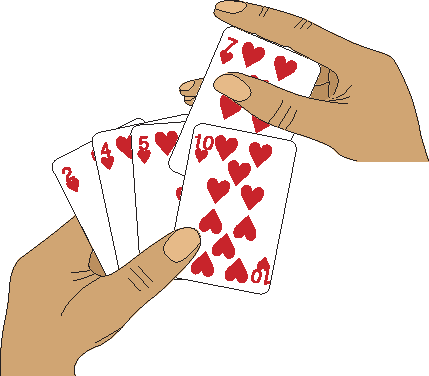
\includegraphics{算法导论第四版插图/第二章/插入排序打牌示意图.pdf}
    \caption{使用插入排序对手中的牌进行排序}
    \label{fig:使用插入排序对手中的牌进行排序}
\end{figure}

插入排序的伪代码在下一页上给出,它被称为INSERTION-SORT过程。它接受两个参数:包含要排序的值的数组和要排序的值的数量。这些值占据数组的位置,我们用表示。当INSERTION-SORT过程结束时,数组包含原始的值,但按排序顺序排列。

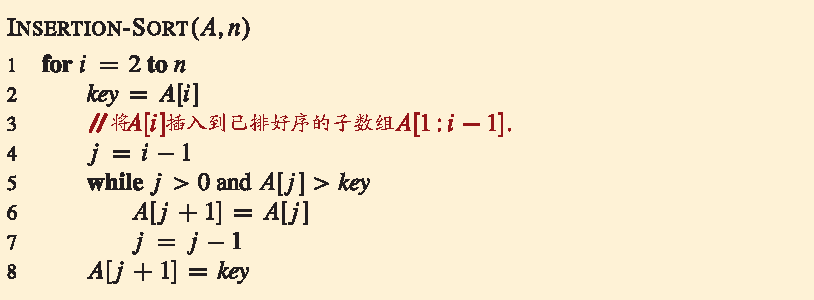
\includegraphics{算法导论第四版插图/第二章/插入排序伪代码.pdf}

\textbf{循环不变量和插入排序的正确性}

\begin{figure}[htbp]
    \centering
    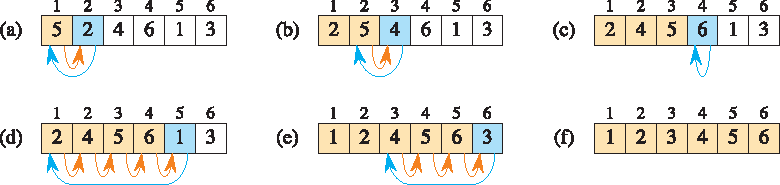
\includegraphics{算法导论第四版插图/第二章/插入排序过程示意图.pdf}
    \caption{INSERTION-SORT$(A,n)$的操作,其中$A$最初包含序列$langle 5,2,4,6,1,3 \rangle$以及有$n = 6$。数组索引出现在矩形上方,数组位置中存储的值出现在矩形内部。(a)-(e) 行1-8的\textbf{for}循环迭代。在每次迭代中,蓝色矩形中存放着从$A[i]$中取出的$key$,该$key$与行5中其左边的棕色矩形中的值进行比较。橙色箭头显示在行6中向右移动一个位置的数组值,蓝色箭头指示$key$在行8中移动到的位置。(f) 最终排序的数组。}
    \label{fig:插入排序过程示意图}
\end{figure}

图\ref{fig:插入排序过程示意图}展示了该算法如何对初始序列$\langle 5,2,4,6,1,3\rangle$的数组$A$进行排序。索引$i$表示正在插入到手中的“当前卡片”。在每次由$i$索引的\textbf{for}循环的开始时,子数组(数组的连续部分)$A[1:i-1]$(即$A[1]$到$A[i-1]$)构成当前已排序的手牌,而剩余的子数组$A[i+1:n]$(元素$A[i+1]$到$A[n]$)对应于仍留在桌上的牌堆。实际上,元素$A[1:i-1]$是最初在位置1到$i-1$上的元素,但现在以排序顺序排列。我们将$A[1:i-1]$的这些属性正式陈述为一个循环不变量:

\begin{tcolorbox}
在第 1-8 行的 \textbf{for} 循环的每次迭代开始时,子数组 $A[1:i-1]$ 由原来在 $A[1:i-1]$ 中的元素组成,但已经按序排列。
\end{tcolorbox}

循环不变量主要用来帮助我们理解算法的正确性。关于循环不变式,我们必须证明三条性质:

\textbf{初始化}:循环的第一次迭代之前,它为真。

\textbf{保持}:如果循环的某次迭代之前它为真,那么下次迭代之前它仍为真。

\textbf{终止}:在循环终止时,循环不变量(通常会包含循环终止的原因)为我们提供一个有用的性质,该性质有助于证明算法是正确的。

当前两条性质成立时,在循环的每次迭代之前循环不变量为真。(当然,为了证明循环不变量在每次迭代之前保持为真,我们完全可以使用不同于循环不变量本身的其他已证实的事实。)注意,这类似于数学归纳法,其中为了证明某条性质成立,需要证明一个基本情况和一个归纳步骤。这里,证明第一次迭代之前循环不变量成立对应于基本情况,证明从一次迭代到下一次迭代不变式成立对应于归纳步骤。

第三条性质也许是最重要的,因为我们将使用循环不变量来证明正确性。通常,我们和导致循环终止的条件一起使用循环不变量。终止性不同于我们通常使用数学归纳法的做法,在归纳法中,归纳步骤是无限地使用的,这里当循环终止时,停止``归纳''。

让我们看看对于插入排序,如何证明这些性质成立。

\textbf{初始化}:首先证明在第一次循环迭代之前(当$i=2$时),循环不变量成立。所以子数组$A[1:i-1]$仅由单个元素$A[1]$组成,实际上就是$A[1]$中原来的元素。而且该子数组是排序好的(毕竟,只包含一个元素的子数组怎么样才不是已经排好序的呢?)。这表明第一次循环迭代之前循环不变量成立。

\textbf{保持}:其次处理第二条性质:证明每次迭代保持循环不变量。非形式化地, \textbf{for} 循环体的第 4-7 行将 $A[i-1]$、$A[i-2]$、$A[i-3]$等向右移动一个位置,直到找到 $A[i]$ 的适当位置,第 8 行将 $A[i]$ 的值插入该位置。这时子数组 $A[1:i]$ 由原来在 $A[1:i]$ 中的元素组成,但已按序排列。那么对 \textbf{for} 循环的下一次迭代增加$i$将保持循环不变量。

第二条性质的一种更形式化的处理要求我们对第 5-7 行的 \textbf{while} 循环给出并证明一个循环不变量。然而,这里我们不愿陷入形式主义的困境,而是依赖以上非形式化的分析来证明第二条性质对外层循环成立。

\textbf{终止}:最后研究在循环终止时发生了什么。循环变量$i$从2开始,每次迭代增加1。一旦第1行代码的$i$的值超过了$n$,循环就将终止。也就是循环会在$i=n+1$时终止。在循环不变式的表述中将$i$用$n+1$代替,我们有:子数组 $A[1:n]$ 由原来在 $A[1:n]$ 中的元素组成,但已按序排列。注意到,子数组 $A[1:n]$ 就是整个数组,我们推断出整个数组已排序。因此算法正确。

在本章后面以及其他章中,我们将采用这种循环不变式的方法来证明算法的正确性。

\textbf{伪代码中的一些约定}

\begin{itemize}
    \item 缩进表示块结构。例如,第 1 行开始的 \textbf{for} 循环体由第 2-8 行组成,第 5 行开始的 \textbf{while} 循环体包含第 6-7 行但不包含第 8 行。我们的缩进风格也适用于 \textbf{if-else} 语句。采用缩进来代替常规的块结构标志,如 \textbf{begin} 和 \textbf{end} 语句,可以大大提高代码的清晰性。
    \item \textbf{while}、\textbf{for} 与 \textbf{repeat-until} 等循环结构以及 \textbf{if-else} 等条件结构与C、C++、Java、Python和JavaScript中的那些结构具有类似的解释。不像某些出现于C++、Java和JavaScript中的情况,本书中在退出循环后,循环计数器保持其值。因此,紧接在一个 \textbf{for} 循环后,循环计数器的值就是第一个超出 \textbf{for} 循环界限的那个值。在证明插入排序的正确性时,我们使用了该性质。第 1 行的 \textbf{for} 循环头为 \textbf{for} $i=2$ \textbf{to} $n$,所以,当该循环终止时,$i=n+1$。当一个 \textbf{for} 循环每次迭代增加其循环计数器时,我们使用关键词\textbf{to}。当一个\textbf{for}循环每次迭代减少其循环计数器时,我们使用关键词 \textbf{downto} 。当循环计数器以大于 1 的一个量改变时,该改变量跟在可选关键词 \textbf{by} 之后。
    \item 符号``//''表示该行后面部分是个注释。
    \item 变量(例如$i$,$j$和$key$)都是给定过程的局部变量。我们在不明确说明的情况下,不使用全局变量。
    \item 我们通过在方括号中指定数组名后跟索引来访问数组元素。例如,$A[i]$表示数组$A$的第$i$个元素。

    尽管许多编程语言对数组采用从0开始的索引(0是最小有效索引),但我们选择最清晰易懂的索引方案供人类读者理解。因为人们通常从1开始计数,而不是从0开始,所以本书中的大多数(但不是全部)数组使用从1开始的索引。为了明确一个特定算法是基于0索引还是1索引,我们会明确指定数组的边界。如果你正在使用一个我们用1索引指定的算法,但你正在使用强制使用0索引的编程语言(如C、C++、Java、Python或JavaScript)编写代码,那么你应该获得可以适应的荣誉。你可以选择始终从每个索引中减去1,或者为每个数组分配一个额外的位置,并忽略位置0。
    
    符号“:”表示子数组。因此,$A[i:j]$表示由元素$A[i],A[i+1],\cdots,A[j]$组成的$A$的子数组。我们还使用这个符号来表示数组的边界,就像我们之前讨论数组$A[1:n]$时所做的那样。
    \item 通常,我们将复合数据组织成对象,对象由属性组成。我们使用许多面向对象编程语言中的语法来访问特定的属性:对象名称,后跟一个点,再后跟属性名称。例如,如果一个对象$x$具有属性$f$,我们用$x.f$表示该属性。

    我们将表示数组或对象的变量视为指向表示数组或对象的数据的指针(在某些编程语言中称为引用)。对于对象$x$的所有属性$f$,将$y = x$设置后,$y.f$将等于$x.f$。此外,如果我们现在设置$x.f = 3$,那么之后不仅$x.f$等于3,$y.f$也等于3。换句话说,在赋值$y = x$之后,$x$和$y$指向同一个对象。这种处理数组和对象的方式与大多数现代编程语言一致。
    
    我们的属性表示法可以"级联"。例如,假设属性$f$本身是指向某种具有属性$g$的对象的指针。那么表示法$x.f.g$隐式地被表示为$(x.f).g$。换句话说,如果我们已经将$y = x.f$赋值,那么$x.f.g$和$y.g$是相同的。
    
    有时指针可能不指向任何对象。在这种情况下,我们给它一个特殊的值NIL。
    \item 我们通过值传递方式将参数传递给过程:被调用的过程接收到参数的自己副本,如果它对参数进行赋值,调用过程不会看到这个变化。当对象被传递时,表示对象的数据的指针被复制,但对象的属性不会被复制。例如,如果$x$是一个被调用过程的参数,被调用过程中的赋值操作$x=y$对调用过程是不可见的。然而,如果调用过程与$x$指向同一个对象,则赋值操作$x.f=3$是可见的。类似地,数组是通过指针传递的,因此传递的是数组的指针而不是整个数组,对单个数组元素的更改对调用过程是可见的。再次强调,大多数当代编程语言都是以这种方式工作的。
    \item \textbf{return}语句立即将控制权转回调用过程中的调用点。大多数\textbf{return}语句还接受一个值作为返回给调用者的结果。我们的伪代码与许多编程语言不同之处在于,我们允许在单个\textbf{return}语句中返回多个值,而不需要创建对象将它们打包在一起。
    \item 布尔运算符``and''和``or''具有短路求值的特性。也就是说,对于表达式``$x$ and $y$'',首先求值$x$。如果$x$的值为\textbf{FALSE},则整个表达式无法为\textbf{TRUE},因此不会对$y$进行求值。另一方面,如果$x$的值为\textbf{TRUE},则必须对$y$进行求值以确定整个表达式的值。类似地,在表达式``$x$ or $y$''中,只有当$x$的值为\textbf{FALSE}时才会对$y$进行求值。短路求值的运算符使我们能够编写布尔表达式,例如``$x$ != NIL and $x.f=y$'',而无需担心当$x$为NIL时对``$x.f$''的求值会发生什么。
    \item 关键字\textbf{error}表示发生了错误,因为调用过程的条件不满足,所以过程立即终止。调用过程负责处理错误,因此我们不指定要采取的具体操作。
\end{itemize}


\section{分析算法}

分析算法的含义已经演变为预测算法所需的资源。你可能考虑到的资源包括内存、通信带宽或能量消耗。然而,最常见的情况是你会希望衡量计算时间。如果你分析一个问题的多个候选算法,你可以找出最高效的算法。可能会有不止一个可行的候选算法,但在这个过程中通常可以排除一些较差的算法。

在你分析算法之前,你需要一个它运行的技术模型,包括该技术的资源以及一种表示它们成本的方法。本书的大部分内容假设计算机程序的实现技术是通用的单处理器随机访问机(RAM)模型,同时假设算法以计算机程序的形式实现。在RAM模型中,指令一个接一个地执行,没有并发操作。RAM模型假设每条指令的执行时间与其他指令相同,并且每次数据访问(使用变量的值或存储到变量中)的时间与其他数据访问相同。换句话说,在RAM模型中,每条指令或数据访问都需要固定的时间,即使是对数组的索引操作也是如此。

严格来说,我们应该准确地定义RAM模型中的指令及其成本。然而,这样做将变得冗长,并且对算法设计和分析的洞察力帮助不大。然而,我们必须小心不要滥用RAM模型。例如,如果RAM模型中有一个排序的指令,那么你可以在一步中完成排序。这样的RAM是不现实的,因为真实计算机中不存在这样的指令。因此,我们的指导是真实计算机的设计方式。RAM模型包含在真实计算机中常见的指令:算术运算(如加法、减法、乘法、除法、取余、取整、取上整)、数据移动(加载、存储、复制)和控制(条件和无条件分支、子程序调用和返回)。

RAM模型中的数据类型包括整数、浮点数(用于存储实数近似值)和字符。真实计算机通常没有单独的数据类型来表示布尔值TRUE和FALSE。相反,它们经常测试一个整数值是否为0(FALSE)或非零(TRUE),就像在C语言中一样。尽管在本书中我们通常不关心浮点数的精度(许多数字在浮点数中无法精确表示),但对于大多数应用程序来说,精度至关重要。我们还假设每个数据字的位数有一个限制。例如,在处理大小为$n$的输入时,我们通常假设整数由$c\log 2n$位表示,其中$c \ge 1$为某个常数。我们要求$c \ge 1$以便每个字可以容纳$n$的值,使我们能够索引各个输入元素,并限制$c$为一个常数,以避免字大小任意增长。(如果字大小可以任意增长,我们可以在一个字中存储大量数据,并在常数时间内对其进行操作,这是一个不现实的场景。)

实际计算机包含未在上述列表中列出的指令,这些指令在RAM模型中代表了一个灰色区域。例如,指数运算是否是一个常数时间的指令?一般情况下,不是的:计算$x^n$,其中$x$和$n$是一般整数,通常需要时间与$n$的对数成比例(参见第934页上的方程式(31.34)),而且你必须担心结果是否适合计算机字中。然而,如果$n$是一个精确的2的幂,指数运算通常可以视为一个常数时间的操作。许多计算机具有"左移"指令,该指令在常数时间内将整数的位向左移动$n$位。在大多数计算机中,将整数的位左移1位等同于乘以2,因此将位左移$n$位等同于乘以$2^n$。因此,只要$n$不超过计算机字的位数,这些计算机可以通过将整数1左移$n$位来在1个常数时间指令内计算$2^n$。我们将尽量避免RAM模型中的这种灰色区域,并将计算$2^n$和乘以$2^n$视为常数时间的操作,前提是结果足够小以适应计算机字中。

RAM模型没有考虑到在当代计算机中普遍存在的内存层次结构。它既没有模拟缓存,也没有模拟虚拟内存。几种其他计算模型试图考虑内存层次效应,这在实际机器上的真实程序中有时非常重要。本书的第11.5节和一些问题考察了内存层次效应,但在大部分情况下,本书的分析并不考虑这些效应。包含内存层次结构的模型比RAM模型复杂得多,因此使用起来可能会很困难。此外,RAM模型的分析通常对实际机器上的性能预测非常准确。

虽然通常在RAM模型中分析算法是直接的,但有时也可能很具有挑战性。你可能需要运用数学工具,如组合学、概率论、代数灵活性以及识别公式中最重要项的能力。因为算法可能对每个可能的输入表现不同,我们需要一种方式来用简单易懂的公式总结其行为。

\textbf{插入排序的分析}

插入排序(INSERTION-SORT)过程需要多长时间?一种方法是在你的计算机上运行它并计时运行时间。当然,你首先需要用一种真实的编程语言实现它,因为无法直接运行我们的伪代码。这样的定时测试会告诉你什么?你将了解插入排序在你特定的计算机上、特定的输入下、你创建的特定实现中、你运行的特定编译器或解释器、你链接的特定库以及与你的定时测试同时运行的特定后台任务(例如检查网络上的传入信息)下运行所需的时间。如果你再次在相同的输入上在你的计算机上运行插入排序,你甚至可能得到不同的定时结果。从仅在一个计算机上的一种插入排序实现以及一个输入上运行,如果你给它一个不同的输入、在不同的计算机上运行它,或者用不同的编程语言实现它,你能确定有关插入排序运行时间的什么呢?并不多。我们需要一种预测的方法,能够根据新的输入来预测插入排序所需的时间。

与其计时运行插入排序,甚至进行多次运行,我们可以通过分析算法本身来确定所需时间。我们将研究它执行伪代码的次数以及每行伪代码的运行时间。我们首先会得出一个精确但复杂的运行时间公式。然后,我们将使用一种方便的符号表示法,提取公式的重要部分,以便比较解决同一问题的不同算法的运行时间。

我们如何分析插入排序?首先,让我们承认运行时间取决于输入。对于排序一千个数字所需的时间比排序三个数字所需的时间长,并不令人感到惊讶。此外,相同大小的两个输入数组的插入排序可能需要不同的时间,这取决于它们的排序程度。尽管运行时间可能取决于输入的许多特征,但我们将重点关注已被证明具有最大影响的特征,即输入的大小,并将程序的运行时间描述为输入大小的函数。为此,我们需要更仔细地定义"运行时间"和"输入大小"这些术语。我们还需要明确我们是在讨论引发最坏情况行为、最好情况行为还是其他情况下的运行时间。

输入大小的最佳概念取决于所研究的问题。对于许多问题,例如排序或计算离散傅里叶变换,最自然的度量方式是输入中项目的数量--例如,正在排序的项目数$n$。对于许多其他问题,例如两个整数的乘法,输入大小的最佳度量是表示输入所需的总位数(采用普通二进制表示法)。有时,用一个以上的数字描述输入的大小更加合适。例如,如果算法的输入是一个图形,通常通过图中顶点的数量和边的数量来表征输入的大小。我们将在研究的每个问题中指明使用的输入大小度量方式。

算法在特定输入上的运行时间是执行的指令和数据访问次数。我们应该如何计算这些开销应该独立于任何特定计算机,但在RAM模型的框架内进行。暂时采用以下观点。执行我们的伪代码的每行都需要恒定的时间。一行可能比另一行需要更多或更少的时间,但我们假设第$k$行的每次执行都需要$c_k$的时间,其中$c_k$是一个常数。这个观点与RAM模型一致,也反映了伪代码在大多数实际计算机上的实现方式。

让我们分析插入排序过程。如前所述,我们将首先设计一个精确的公式,其中使用了输入大小和所有语句的成本$c_k$。然而,这个公式可能会变得混乱。然后,我们将切换到一种更简洁、更易于使用的简化符号表示法。这种简化表示法清楚地说明了如何比较算法的运行时间,特别是随着输入大小的增加。

为了分析INSERTION-SORT过程,让我们在接下来的页面上查看它,记录每个语句的时间成本和每个语句的执行次数。对于每个$i=2,3,\cdots,n$,设$t_i$表示在第5行的while循环测试中对于该$i$值执行的次数。当for循环或while循环以通常的方式退出(因为循环头中的测试结果为FALSE),测试的执行次数比循环体多一次。由于注释不是可执行语句,请假设它们不占用时间。

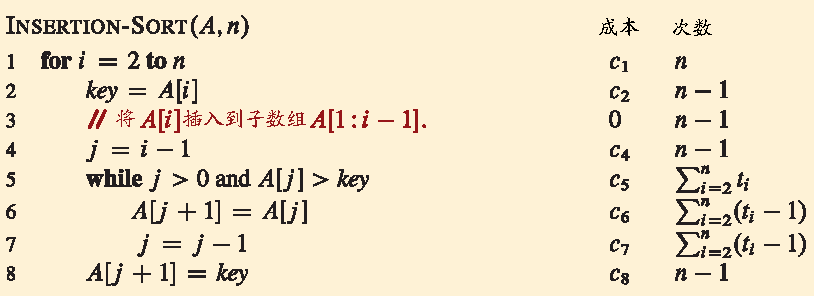
\includegraphics{算法导论第四版插图/第二章/插入排序时间复杂度的代码.pdf}

算法的运行时间是每个语句执行时间的总和。一个执行需要$c_k$步并且执行$m$次的语句对总运行时间的贡献为$c_km$。我们通常用$T(n)$表示算法在大小为$n$的输入上的运行时间。要计算$T(n)$,即INSERTION-SORT在给定输入值上的运行时间,我们将成本和次数两列的乘积相加,得到

\begin{equation*}
\begin{aligned}
T(n)= & c_1 n+c_2(n-1)+c_4(n-1)+c_5 \sum_{i=2}^n t_i+c_6 \sum_{i=2}^n\left(t_i-1\right) \\
& +c_7 \sum_{i=2}^n\left(t_i-1\right)+c_8(n-1) .
\end{aligned}
\end{equation*}

即使对于给定大小的输入,算法的运行时间可能取决于给定的该大小的输入。例如,在INSERTION-SORT中,最佳情况是数组已经排序好。在这种情况下,每次执行第5行时,$key$的值(即最初在$A[i]$中的值)已经大于或等于$A[1:i-1]$中的所有值,因此在第5行的第一次测试中,循环将总是退出。因此,我们有$t_i=1$对于$i=2,3,\cdots,n$,最佳情况的运行时间由以下公式给出

\begin{equation}
\begin{aligned}
T(n) & =c_1 n+c_2(n-1)+c_4(n-1)+c_5(n-1)+c_8(n-1) \\
& =\left(c_1+c_2+c_4+c_5+c_8\right) n-\left(c_2+c_4+c_5+c_8\right) .
\end{aligned}
\end{equation}

我们可以将这个运行时间表示为$an+b$,其中$a$和$b$是依赖于语句成本$c_k$的常数(其中$a = c_1 + c_2 + c_4 + c_5 + c_8$,$b = c_2 + c_4 + c_5 + c_8$)。因此,运行时间是$n$的线性函数。

最坏情况出现在数组按逆序排列的情况下,即初始时按降序排列。该过程必须将每个元素$A[i]$与整个已排序子数组$A[1:i-1]$中的每个元素进行比较,因此对于$i=2,3,\cdots,n$,$t_i = i$。(在第5行,该过程发现每次$A[j] > key$,并且while循环仅在$j$达到0时退出。)注意到

\begin{equation*}
\begin{aligned}
\sum_{i=2}^n i & =\left(\sum_{i=1}^n i\right)-1 \\
& =\frac{n(n+1)}{2}-1
\end{aligned}
\end{equation*}

和

\begin{equation*}
\begin{aligned}
\sum_{i=2}^n(i-1) & =\sum_{i=1}^{n-1} i \\
& =\frac{n(n-1)}{2}
\end{aligned}
\end{equation*}

我们可以看到插入排序在最坏情况下的运行时间是

\begin{equation}
\begin{aligned}
T(n)= & c_1 n+c_2(n-1)+c_4(n-1)+c_5\left(\frac{n(n+1)}{2}-1\right) \\
& +c_6\left(\frac{n(n-1)}{2}\right)+c_7\left(\frac{n(n-1)}{2}\right)+c_8(n-1) \\
= & \left(\frac{c_5}{2}+\frac{c_6}{2}+\frac{c_7}{2}\right) n^2+\left(c_1+c_2+c_4+\frac{c_5}{2}-\frac{c_6}{2}-\frac{c_7}{2}+c_8\right) n \\
& -\left(c_2+c_4+c_5+c_8\right)
\end{aligned}
\end{equation}

我们可以将最坏情况的运行时间表示为$an^2+bn+c$,常数$a$,$b$和$c$依赖于语句代价$c_k$(现在,$a=c_5 / 2+c_6 / 2+c_7 / 2$,$b=c_1+c_2+c_4+c_5 / 2-c_6 / 2-c_7 / 2+c_8$以及$\left.c=-\left(c_2+c_4+c_5+c_8\right)\right)$)。这个运行时间是$n$的平方函数。

一般来说,对于给定输入,插入排序的运行时间是固定的,尽管我们可能会看到某些有趣的``随机''算法,对于这些算法而言,对于固定的输入,算法的行为可能会变化。

\textbf{最坏情况和平均情况的分析}

我们对插入排序的分析同时考虑了最好情况(即输入数组已经排序)和最坏情况(即输入数组按逆序排列)。然而,在本书的剩余部分,我们通常(但不总是)只关注寻找最坏情况的运行时间,即任意大小为$n$的输入的最长运行时间。为什么呢?以下是三个原因:

\begin{itemize}
    \item 算法的最坏情况运行时间为任何输入提供了一个运行时间的上界。如果你知道最坏情况运行时间,那么你可以确保算法永远不会花费更长的时间。你不需要对运行时间进行猜测,并希望它不会变得更糟。这一特性对于实时计算尤其重要,因为在实时计算中,操作必须在截止日期之前完成。
    \item 对于某些算法,最坏情况经常发生。例如,在搜索数据库中的特定信息时,搜索算法的最坏情况通常发生在数据库中不存在该信息的情况下。在某些应用中,对不存在信息的搜索可能很频繁。
    \item "平均情况"通常与最坏情况差不多糟糕。假设你在一个包含 $n$ 个随机选择数字的数组上运行插入排序。确定将元素 $A[i]$ 插入子数组 $A[1:i-1]$ 中的位置需要多长时间?平均而言,$A[1:i-1]$ 的一半元素小于 $A[i]$,另一半元素大于 $A[i]$。因此,平均而言,$A[i]$ 与子数组 $A[1:i-1]$ 的一半元素进行比较,所以 $t_i$ 大约为 $i/2$。因此,结果的平均情况运行时间是输入规模的二次函数,就像最坏情况运行时间一样。
\end{itemize}

在某些特定情况下,我们对算法的平均情况运行时间感兴趣。我们将在本书中看到概率分析技术应用于各种算法。平均情况分析的范围有限,因为对于特定问题的“平均”输入可能不明确。通常,我们假设给定大小的所有输入等可能出现。实际上,这个假设可能被违反,但我们有时可以使用随机化算法,通过进行随机选择来进行概率分析并得出预期的运行时间。我们在第5章和其他几个后续章节中更详细地探讨随机化算法。

\textbf{增长量级}

为了简化对INSERTION-SORT过程的分析,我们使用了一些简化的抽象概念。首先,我们忽略了每个语句的实际成本,而使用常数$c_k$来表示这些成本。然而,方程(2.1)和(2.2)中的最佳情况和最坏情况的运行时间相当复杂。这些表达式中的常数提供了比我们实际需要的更多细节。这就是为什么我们还将最佳情况的运行时间表示为$an+b$,其中$a$和$b$是依赖于语句成本$c_k$的常数,以及为什么我们将最坏情况的运行时间表示为$an^2+bn+c$,其中$a$,$b$和$c$是依赖于语句成本的常数。因此,我们不仅忽略了实际的语句成本,还忽略了抽象的成本$c_k$。

现在让我们再做一个简化的抽象:我们真正关心的是运行时间的增长率或阶数。因此,我们只考虑公式的主要项(例如,$an^2$),因为对于较大的$n$值来说,次要项相对不重要。我们还忽略主要项的常数系数,因为对于较大的输入,常数因子比增长率在确定计算效率时要不重要。对于插入排序的最坏情况运行时间,当我们忽略次要项和主要项的常数系数时,只剩下主要项的$n^2$因子。这个因子$n^2$是运行时间中最重要的部分。例如,假设一个算法在特定机器上在大小为$n$的输入上花费$n^2/100 + 100n + 17$微秒。尽管$n^2$项的系数$1/100$和$n$项的系数100相差了四个数量级,但是一旦$n$超过10000,$n^2/100$项就主导了$100n$项。尽管10000可能看起来很大,但它比一个普通城镇的人口要小。许多现实世界的问题具有更大的输入规模。

为了突出运行时间的增长率,我们使用了特殊的符号,使用希腊字母$\Theta$(theta)。我们表示插入排序的最坏情况运行时间为$\Theta(n^2)$。我们还表示插入排序的最好情况运行时间为$\Theta(n)$。暂时将$\Theta$记号视为表示"当$n$很大时大致成正比"的方式,因此$\Theta(n^2)$表示"当$n$很大时大致与$n^2$成正比",$\Theta(n)$表示"当$n$很大时大致与$n$成正比"。我们将在本章中非正式地使用$\Theta$记号,并在第3章中精确定义它。

通常情况下,如果一个算法的最坏情况运行时间具有较低的增长阶数,我们会认为该算法比另一个算法更高效。由于常数因子和次要项的影响,具有较高增长阶数的算法在小规模输入上可能比具有较低增长阶数的算法花费更少的时间。但是在足够大的输入上,一个最坏情况运行时间为$\Theta(n^2)$的算法,例如,其最坏情况下的时间比一个最坏情况运行时间为$\Theta(n^3)$的算法更少。无论$\Theta$-notation中隐藏了哪些常数,总是存在某个数$n_0$,使得对于所有输入大小$n\ge n_0$,$\Theta(n^2)$算法在最坏情况下击败$\Theta(n^3)$算法。

\section{设计算法}

你可以选择从广泛的算法设计技术中进行选择。插入排序使用增量方法:对于每个元素$A[i]$,将其插入到子数组$A[1:i]$的适当位置,已经对子数组$A[1:i-1]$进行了排序。

本节介绍了另一种设计方法,称为``分治法'',我们将在第4章中详细探讨。我们将使用分治法设计一个排序算法,其最坏情况运行时间远远小于插入排序。使用遵循分治法的算法的一个优点是,分析其运行时间通常是直接的,使用的技术我们将在第4章中探讨。

\subsection{分治策略}

许多有用的算法具有递归的结构:为了解决一个给定的问题,它们会递归(调用自身)一次或多次来处理紧密相关的子问题。这些算法通常遵循分治法:它们将问题分解为几个与原始问题类似但规模较小的子问题,递归地解决这些子问题,然后将这些解合并以创建原始问题的解决方案。

在分治法中,如果问题足够小(基本情况),则直接解决它而不进行递归。否则(递归情况),您执行三个特定的步骤:

\textbf{分解}原问题为若干子问题,这些子问题是原问题的规模较小的实例。

\textbf{解决}这些子问题,递归地求解各子问题。然而,若子问题的规模足够小,则直接求解。

\textbf{合并}这些子问题的解成原问题的解。

\textbf{归并排序}算法严格遵照了以上的分治策略。在每一个步骤,归并排序会对子数组$A[p:r]$进行排序。归并排序从整个数组$A[1:n]$开始,一直递归下降到越来越小的子数组。下面就是归并排序的操作过程:

\textbf{分解}:将待排序的子数组 $A[p:r]$ 分成两个相邻的子数组,每个子数组的大小都是原数组的一半。为此,计算子数组 $A[p:r]$ 的中点 $q$(取 $p$ 和 $r$ 的平均值),并将 $A[p:r]$ 分成子数组 $A[p:q]$ 和 $A[q+1:r]$。

\textbf{解决}:通过使用归并排序对两个子数组 $A[p:q]$ 和 $A[q+1:r]$ 进行递归排序来征服。

\textbf{合并}:通过将两个已排序的子数组 $A[p:q]$ 和 $A[q+1:r]$ 合并回 $A[p:r]$,得到排序好的答案。

当待排序的子数组 $A[p:r]$ 仅包含1个元素时,即 $p$ 等于 $r$ 时,递归“bottoms out”(到达基本情况)。正如我们在INSERTION-SORT循环不变式的初始化参数中指出的那样,只包含一个元素的子数组总是有序的。

归并排序算法的关键操作发生在“合并”步骤中,即合并两个相邻的已排序子数组。合并操作是由下一页上的辅助过程 MERGE$(A,p,q,r)$ 执行的,其中 $A$ 是一个数组,$p$、$q$ 和 $r$ 是数组的索引,满足 $p\le q < r$。该过程假设相邻的子数组 $A[p:q]$ 和 $A[q+1:r]$ 已经递归地排序好了。它将这两个已排序的子数组合并成一个单独的已排序子数组,取代当前的子数组 $A[p:r]$。

为了理解MERGE过程的工作原理,让我们回到我们之前提到的纸牌游戏的情景。假设你在桌子上有两堆面朝上的纸牌。每堆纸牌都是有序的,最小值的牌在顶部。你希望将这两堆纸牌合并成一堆有序的纸牌,放在桌子上面朝下。基本步骤包括选择两堆面朝上纸牌中较小的一张牌,将其从所属的堆中移除(暴露出新的顶部牌),然后将这张牌面朝下放在输出堆上。重复这个步骤,直到其中一堆纸牌为空,这时你可以将剩下的一堆纸牌整体翻转并放在输出堆上。

我们来思考一下合并两堆有序纸牌需要多长时间。每个基本步骤都需要固定的时间,因为你只是比较两张顶部的纸牌。如果你开始时的两堆有序纸牌分别有$n/2$张牌,那么基本步骤的数量至少为$n/2$(因为在其中一堆被清空时,每张纸牌都被发现比另一堆的某张纸牌小),最多为$n$(实际上最多为$n-1$,因为经过$n-1$个基本步骤后,其中一堆必定为空)。每个基本步骤花费固定的时间,而总的基本步骤数量在$n/2$和$n$之间,因此我们可以说合并操作的时间与$n$大致成正比。也就是说,合并操作的时间复杂度为$\Theta(n)$。

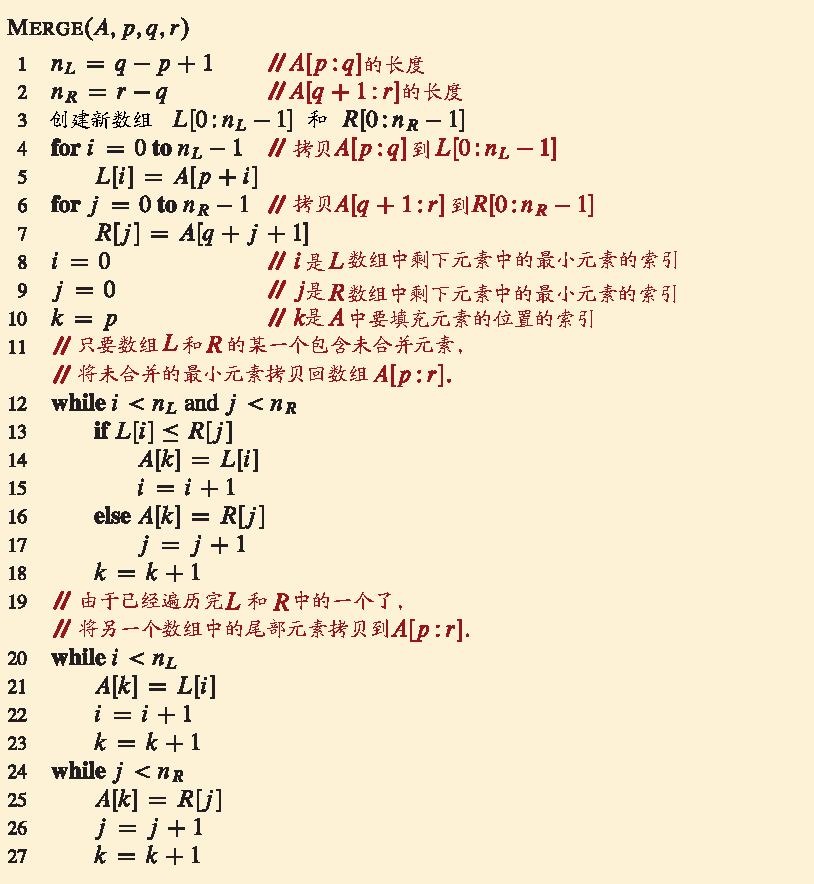
\includegraphics{算法导论第四版插图/第二章/归并过程伪代码.pdf}

具体来说,MERGE过程的工作步骤如下。它将两个子数组$A[p:q]$和$A[q+1:r]$复制到临时数组$L$和$R$("left"和"right"),然后将$L$和$R$中的值合并回$A[p:r]$中。第1行和第2行计算子数组$A[p:q]$和$A[q+1:r]$的长度$n_L$和$n_R$,然后第3行创建具有长度$n_L$和$n_R$的数组$L[0:n_L-1]$和$R[0:n_R-1]$。第4至第5行的for循环将子数组$A[p:q]$复制到$L$,第6至第7行的for循环将子数组$A[q+1:r]$复制到$R$。

\begin{figure}[htbp]
    \centering
    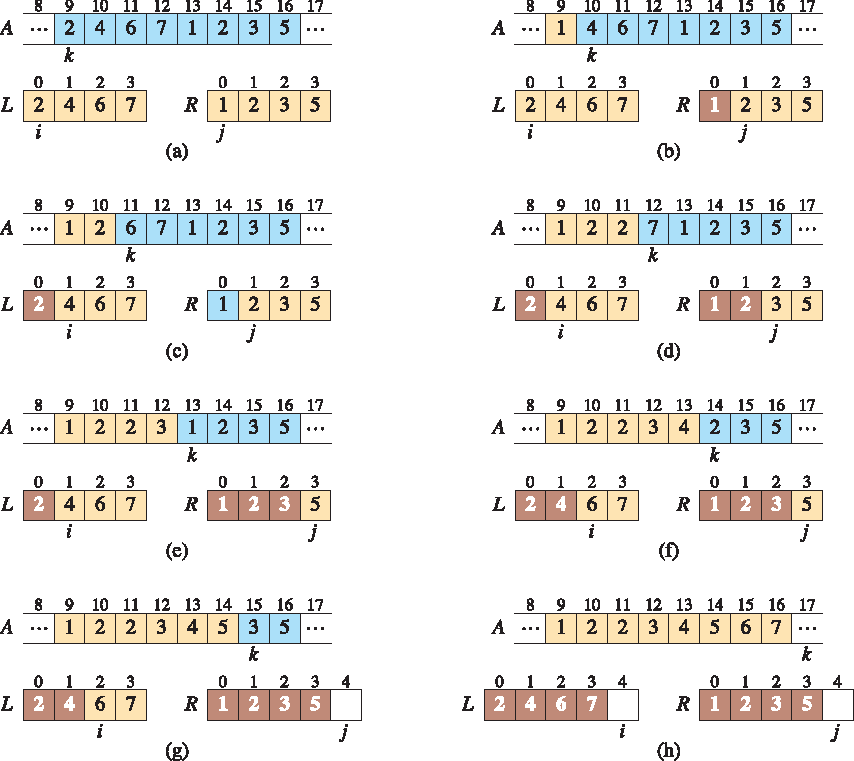
\includegraphics{算法导论第四版插图/第二章/归并过程示意图.pdf}
    \caption{在调用MERGE$(A,9,12,16)$时,循环行8-18中的操作是,当子数组$A[9:16]$包含值$\langle 2,4,6,7,1,2,3,5 \rangle$时进行的。在分配和复制到数组$L$和$R$之后,数组$L$包含$\langle 2,4,6,7 \rangle$,数组$R$包含$\langle 1,2,3,5 \rangle$。$A$中的棕色位置包含它们的最终值,$L$和$R$中的棕色位置包含尚未复制回$A$的值。总体而言,棕色位置始终包含最初在$A[9:16]$中的值。$A$中的蓝色位置包含将要复制的值,$L$和$R$中的深色位置包含已经复制回$A$的值。 (a)-(g)是循环12-18行的每次迭代之前的数组$A$、$L$和$R$以及它们的相应索引$k$、$i$和$j$。在(g)部分,$R$中的所有值都已经复制回$A$($j$等于$R$的长度),因此循环12-18行的while循环终止。(h)是终止时的数组和索引。行20-23的while循环复制回$A$中剩余的$L$和$R$的值,这些值是最初在$A[9:16]$中的最大值。在这里,行20-23将$L[2:3]$复制到$A[15:16]$,并且因为$R$中的所有值已经复制回$A$,所以循环24-27行的while循环迭代0次。此时,$A[9:16]$的子数组已经排序完成。}
    \label{fig:归并过程示意图}
\end{figure}

在图\ref{fig:归并过程示意图}中展示的第8-18行执行基本步骤。循环12-18行重复地在$L$和$R$中找到尚未复制回$A[p:r]$的最小值,并将其复制回去。正如注释所示,索引$k$表示正在填充的$A$的位置,索引$i$和$j$分别表示$L$和$R$中剩余最小值的位置。最终,$L$或$R$中的所有值都被复制回$A[p:r]$,并且此循环终止。如果循环终止是因为已经将$R$的所有值复制回去,即$j$等于$n_R$,那么$i$仍然小于$n_L$,这意味着$L$的一些值尚未复制回去,而这些值是$L$和$R$中最大的值。在这种情况下,循环20-23行将$L$的这些剩余值复制到$A[p:r]$的最后几个位置。因为$j$等于$n_R$,所以循环24-27行的while循环不会执行。如果相反,循环12-18行终止是因为$i$等于$n_L$,则所有的$L$已经被复制回$A[p:r]$,而循环24-27行将$R$的剩余值复制回$A[p:r]$的末尾。

为了证明MERGE过程在$\Theta(n)$的时间内运行,其中$n=r-p-1$,观察到第1-3行和第8-10行每行都需要常数时间,而第4-7行的循环需要$\Theta(n_L+n_R)=\Theta(n)$的时间。要计算第12-18行、20-23行和24-27行的三个while循环的时间,观察到这些循环的每次迭代都将$L$或$R$中的一个值复制回$A$,并且每个值都只复制回$A$一次。因此,这三个循环总共进行了$n$次迭代。由于这三个循环的每次迭代都需要常数时间,所以在这三个循环中总共花费的时间是$\Theta(n)$。

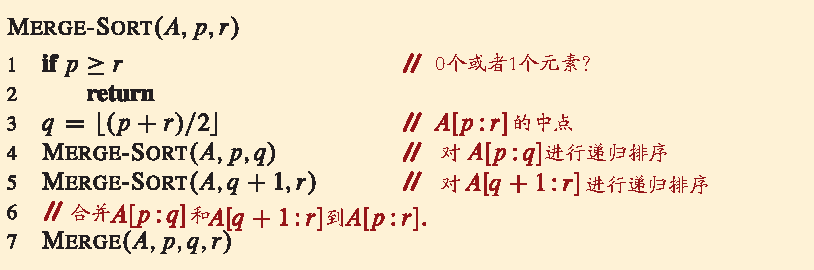
\includegraphics{算法导论第四版插图/第二章/归并排序主程序.pdf}

现在,我们可以将MERGE过程作为合并排序算法中的子程序使用。在下一页上的过程MERGE-SORT$(A,p,r)$对子数组$A[p:r]$中的元素进行排序。如果$p$等于$r$,则子数组只有1个元素,因此已经排序。否则,我们必须有$p < r$,并且MERGE-SORT执行分割、征服和合并步骤。分割步骤简单地计算一个索引$q$,将$A[p:r]$分为两个相邻的子数组:$A[p:q]$,包含$\lceil{n/2}\rceil$个元素,和$A[q+1:r]$,包含$\lfloor{n/2}\rfloor$个元素。初始调用MERGE-SORT$(A,1,n)$对整个数组$A[1:n]$进行排序。

\begin{figure}[htbp]
    \centering
    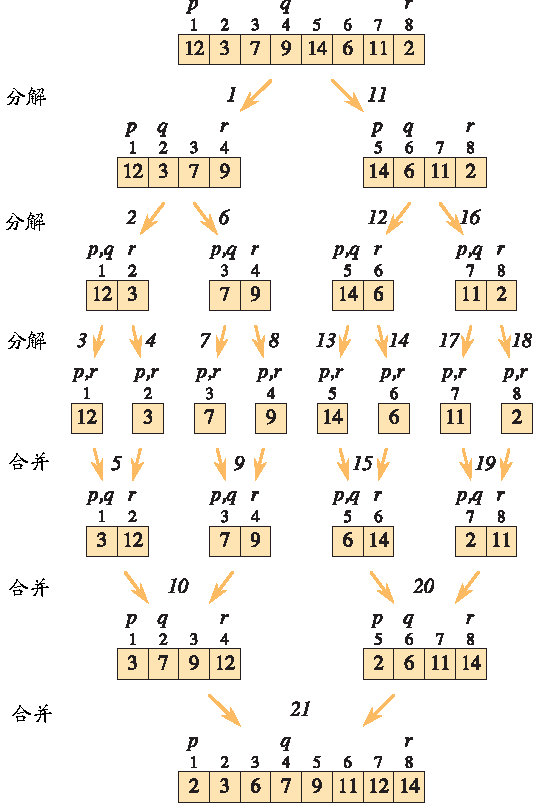
\includegraphics{算法导论第四版插图/第二章/归并排序完整过程示意图.pdf}
    \caption{归并排序在数组长度为8的数组$A$上面的操作过程。数组$A$最开始时是:$\langle{12,3,7,9,14,6,11,2}\rangle$}。每个子数组中的索引$p$、$q$和$r$如图所示。斜体数字表示了MERGE-SORT和MERGE过程的调用顺序,初始调用是MERGE-SORT$(A,1,8)$
    \label{fig:归并排序完整过程示意图}
\end{figure}

图\ref{fig:归并排序完整过程示意图}展示了当$n=8$时该过程的操作,还显示了分割和合并步骤的顺序。该算法递归地将数组分割为包含一个元素的子数组。合并步骤将成对的1元素子数组合并为长度为2的已排序子数组,将它们合并为长度为4的已排序子数组,最终将它们合并为长度为8的最终已排序子数组。如果$n$不是2的精确幂,则某些分割步骤会创建长度相差1的子数组(例如,将长度为7的子数组分割时,一个子数组长度为4,另一个子数组长度为3)。无论合并的两个子数组的长度如何,合并$n$个项的时间复杂度为$\Theta(n)$。

\subsection{分析分治算法}

当一个算法包含递归调用时,通常可以通过递归方程或递归来描述其运行时间,该递归方程描述了算法在较小输入上的运行时间与问题规模$n$上的总体运行时间之间的关系。然后,可以使用数学工具来解决递归方程并提供算法性能的界限。

分治算法的运行时间的递归方程可从基本方法的三个步骤中推导出来。与插入排序类似,假设$T(n)$是规模为n的问题的最坏情况运行时间。如果问题规模足够小,例如$n < n_0$,其中$n_0 > 0$是一个常数,直接的解决方案只需要常数时间,我们将其表示为$\Theta(1)$。假设问题的划分产生了大小为$n/b$的子问题,即原问题大小的$1/b$。对于归并排序,$a$和$b$都是$2$,但是我们将看到其他分治算法中的$a\neq b$。解决一个大小为$n/b$的子问题需要$T(n/b)$的时间,因此解决所有$a$个子问题需要$aT(n/b)$的时间。如果将问题划分成子问题需要$D(n)$的时间,将子问题的解合并成原问题的解需要$C(n)$的时间,我们得到递归关系式

$$
T(n)= \begin{cases}\Theta(1) & \text { if } n<n_0 \\ D(n)+a T(n / b)+C(n) & \text { otherwise }\end{cases}
$$

第4章展示了如何求解以上形式的递归式。

有时候,分治算法中的划分步骤的大小 $n/b$ 不是整数。例如,归并排序将一个大小为 $n$ 的问题划分为大小为 $\lfloor{n/2}\rfloor$ 和 $\lceil{n/2}\rceil$ 的子问题。由于 $\lfloor{n/2}\rfloor$ 和 $\lceil{n/2}\rceil$ 之间的差异最多为 1,对于大的 $n$ 来说,这比将 $n$ 除以 2 的影响要小得多,因此我们会简单地将它们都称为大小为 $n/2$。正如第四章所讨论的那样,忽略 floor 和 ceiling 并不会影响分治递归的解决方案的增长顺序。

我们还要采用的另一个约定是省略递归基的语句,我们将在第四章中更详细地讨论这个问题。原因是基本情况几乎总是 $T(n)=\Theta(1)$,如果 $n < n_0$,其中 $n_0 > 0$ 是一个常数。这是因为算法在常量大小的输入上运行时间是恒定的。采用这种约定可以节省大量的写作时间。

\textbf{归并排序算法的分析}

下面是如何设置归并排序在 $n$ 个数字上的最坏情况运行时间 $T(n)$ 的递归公式:

划分:划分步骤只是计算子数组的中间位置,这需要恒定时间。因此,$D(n)=\Theta(1)$。

解决:递归地解决两个大小为 $n/2$ 的子问题,每个子问题对运行时间的贡献为 $2T(n/2)$(忽略 floor 和 ceiling,如我们所讨论的)。

合并:由于对 $n$ 元素子数组进行合并的 MERGE 过程需要 $\Theta(n)$ 的时间,因此我们有 $C(n)=\Theta(n)$。

当我们将归并排序分析中的函数 $D(n)$ 和 $C(n)$ 相加时,我们正在添加一个 $\Theta(n)$ 的函数和一个 $\Theta(n)$ 的函数。这个和是 $n$ 的线性函数。也就是说,当 $n$ 很大时,它大致与 $n$ 成正比,因此归并排序的划分和合并时间总共为 $\Theta(n)$。将 $\Theta(n)$ 添加到解决步骤中的 $2T(n/2)$ 项中,得到归并排序最坏情况运行时间 $T(n)$ 的递归公式:

\begin{equation}
T(n)=2T(n/2)+\Theta(n)
\end{equation}

第四章介绍了“主定理”,它表明$T(n)=\Theta(n\lg{n})$。与最坏情况运行时间为$\Theta(n^2)$的插入排序相比,归并排序以$n$的因子换取了$\lg n$的因子。因为对数函数增长比任何线性函数都要慢,所以这是一个好的交易。对于足够大的输入,具有$\Theta(n \lg n)$最坏情况运行时间的归并排序优于最坏情况运行时间为$\Theta(n^2)$的插入排序。

我们不需要使用主定理来直观地理解为什么(2.3)的递归解是$T(n) = \Theta(n \lg n)$。为简单起见,假设n是2的幂次方,隐含的基本情况是$n = 1$。那么递归(2.3)本质上是:

\begin{equation}
T(n)= \begin{cases}c_1 & \text { if } n=1 \\ 2 T(n / 2)+c_2 n & \text { if } n>1\end{cases}
\end{equation}

其中常数$c_1 > 0$表示解决大小为1的问题所需的时间,$c_2 > 0$是分割和合并步骤每个数组元素的时间。

\begin{figure}[htbp]
    \centering
    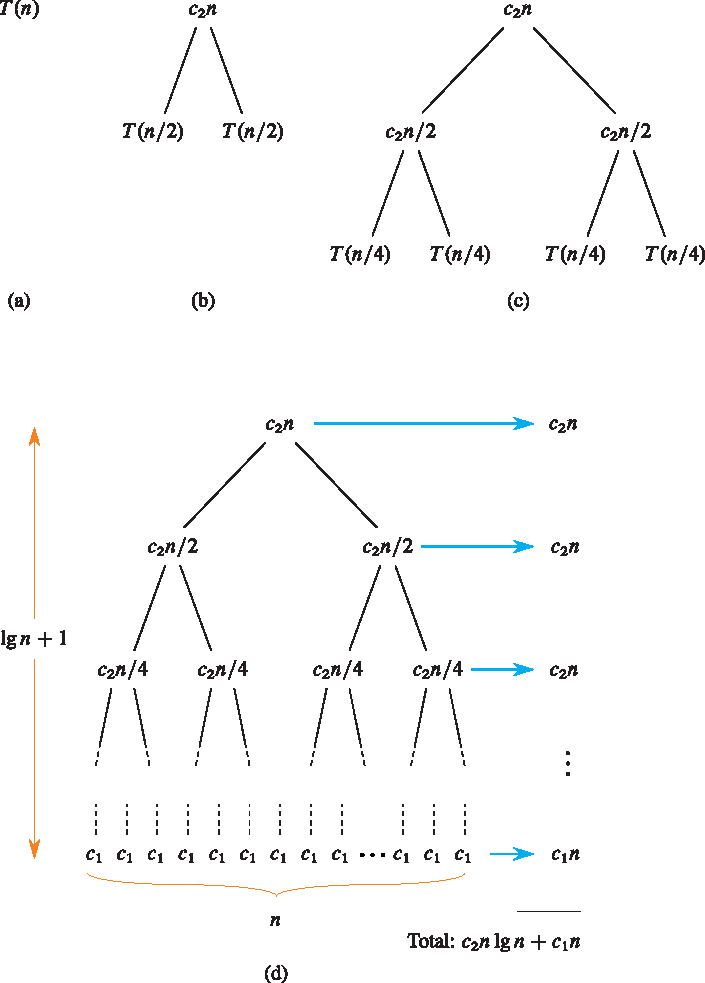
\includegraphics{算法导论第四版插图/第二章/归并排序的递归树示意图.pdf}
    \caption{如何为递归式(2.4)构建递归树。图(a)显示了$T(n)$,在(b)-(d)中逐步扩展以形成递归树。在(d)中完全展开的树有$\lg n + 1$层。叶子节点上面的每个层级共同贡献$c_2n$的总成本,而叶子节点层级则贡献$c_1n$。因此,总成本为$c_2 n \lg n+c_1 n=\Theta(n \lg n)$。}
    \label{fig:归并排序的递归树示意图}
\end{figure}

图\ref{fig:归并排序的递归树示意图}说明了解决递归(2.4)的一种方法。图(a)显示了$T(n)$,图(b)将其扩展为表示递归的等效树。$c_2n$项表示在递归的顶层进行分割和合并的成本,根的两个子树是两个更小的递归$T(n/2)$。图(c)展示了进一步扩展$T(n/2)$的过程,第二层递归中每个节点分割和合并的成本为$c_2 n/2$。继续通过将树中的每个节点展开为由递归确定的组成部分,直到问题大小降至1,每个问题的成本为$c_1$。图(d)显示了得到的递归树。

接下来,将每个层级的成本相加。顶层的总成本为$c_2n$,下一层的总成本为$c_2(n / 2)+c_2(n / 2)=c_2 n$,之后的层级总成本为$c_2(n / 4)+c_2(n / 4)+c_2(n / 4)+c_2(n / 4)=c_2 n$,以此类推。每个层级的节点数是上一层级的两倍,但每个节点仅贡献上一层节点成本的一半。从一个层级到下一个层级,加倍和减半相互抵消,因此每个层级的成本相同:$c_2n$。通常情况下,距离顶部$i$个层级的层级具有$2^i$个节点,每个节点贡献$c_2(n/2^i)$的成本,因此距离顶部第$i$个层级的总成本为$2^i \cdot c_2\left(n / 2^i\right)=c_2 n$。底层具有$n$个节点,每个节点贡献$c_1$的成本,总成本为$c_1n$。

在图\ref{fig:归并排序的递归树示意图}中递归树的总层数是$\lg n+1$,其中$n$是叶子节点的数量,对应于输入大小。一个非正式的归纳论证证明了这个结论。当$n=1$时,基本情况发生,此时树只有1层。由于$\lg 1 = 0$,因此$\lg n + 1$给出了正确的层数。现在假设归纳假设是具有$2^i$个叶子节点的递归树的层数为$\lg 2^i+1=i+1$(因为对于任何$i$值,我们有$\lg 2^i=i$)。因为我们假设输入大小是2的幂次方,所以要考虑的下一个输入大小是$2^{i+1}$。具有$n=2^{i+1}$个叶子节点的树比具有$2^i$个叶子节点的树多1层,因此总层数为$(i+1)+1=\lg{2^{i+1}}+1$。

要计算递归式(2.4)表示的总成本,只需将所有层级的成本相加。递归树有$\lg n + 1$层。叶子节点上面的每个层级成本均为$c_2n$,叶子节点层级成本为$c_1n$,总成本为$c_2 n \lg n + c_1 n = \Theta(n \lg n)$。

\chapter{如何刻画算法的运行时间?}

算法运行时间的增长量级,定义在第2章中,为表征算法效率提供了一种简单的方法,并且还允许我们将其与备选算法进行比较。一旦输入大小$n$足够大,具有$\Theta(n\lg n)$最坏情况运行时间的归并排序将击败具有$\Theta(n^2)$最坏情况运行时间的插入排序。尽管我们有时可以确定算法的确切运行时间,就像第2章中对插入排序所做的那样,但额外的精度很少值得计算。对于足够大的输入,确切运行时间的乘法常数和低阶项被输入大小本身的影响所支配。

当我们考虑输入大小足够大以使仅有运行时间增长量级相关时,我们正在研究算法的渐近效率。也就是说,我们关心的是算法运行时间如何随着输入大小在极限情况下随着输入大小无限增加而增加。通常,渐近效率更高的算法对于除非非常小的输入外都是最佳选择。

本章介绍了几种简化算法渐近分析的标准方法。下一节非正式地介绍了三种最常用的“渐近符号”类型,其中我们已经在$\Theta$符号中看到了一个例子。它还展示了一种使用这些渐近符号来推断插入排序最坏情况运行时间的方法。然后,我们更正式地查看渐近符号,并介绍了本书中使用的几种符号约定。最后一节回顾了在分析算法时经常出现的函数行为。

\section{\texorpdfstring{$O\text{记号,}$}\texorpdfstring{$\Omega\text{记号和}$}\texorpdfstring{$\Theta\text{记号}$}.}

当我们在第二章分析插入排序在最坏情况下的运行时间时,我们是从下面的超级复杂的式子开始的

\begin{equation*}
\begin{aligned}
\left(\frac{c_5}{2}+\right. & \left.\frac{c_6}{2}+\frac{c_7}{2}\right) n^2+\left(c_1+c_2+c_4+\frac{c_5}{2}-\frac{c_6}{2}-\frac{c_7}{2}+c_8\right) n \\
& -\left(c_2+c_4+c_5+c_8\right) .
\end{aligned}
\end{equation*}

然后我们舍弃了低阶项$\left(c_1+c_2+c_4+c_5 / 2-c_6 / 2-c_7 / 2+c_8\right) n$和$c_2+c_4+c_5+c_8$,并忽略了$n^2$的系数$c_5 / 2+c_6 / 2+c_7 / 2$。这只留下了因子$n^2$,我们将其放入$\Theta$符号中,表示为$\Theta(n^2)$。我们使用这种方式来表征算法的运行时间:舍弃低阶项和主导项的系数,并使用一种关注运行时间增长速度的符号表示法。

$\Theta$符号不是唯一的“渐近符号”。在本节中,我们还将看到其他形式的渐近符号。我们首先直观地看一下这些符号,重新审视插入排序以了解如何应用它们。在下一节中,我们将看到我们的渐近符号的正式定义,以及使用它们的约定。

在具体介绍之前,请记住我们将看到的渐近符号是为了表征函数而设计的。恰好我们最感兴趣的函数表示算法的运行时间。但是,渐近符号可以应用于表征算法的其他方面(例如它们使用的空间量),甚至可以应用于与算法毫无关系的函数。

\textbf{$O$记号}

$O$符号表征了函数渐近行为的上限。换句话说,它表示函数的增长速度不会超过某个速率,这个速率基于最高阶项。例如,考虑函数$7 n^3+100 n^2-20 n+6$。它的最高阶项是$7n^3$,因此我们说这个函数的增长速度是$n^3$。因为这个函数的增长速度不会超过$n^3$,所以我们可以写成$O(n^3)$。你可能会惊讶地发现我们也可以写成函数$7 n^3+100 n^2-20 n+6$是$O(n^4)$。为什么呢?因为这个函数的增长速度比$n^4$慢,所以我们说它不会增长得更快。正如你可能猜到的那样,这个函数也是$O(n^5)$、$O(n^6)$等等。更一般地,它是$O(n^c)$,其中$c \ge 3$是任意常数。

\textbf{$\Omega$记号}

$\Omega$符号表征了函数渐近行为的下限。换句话说,它表示函数的增长速度至少和某个速率一样快,这个速率基于最高阶项,就像$O$符号一样。因为函数$7 n^3+100 n^2-20 n+6$中最高阶项的增长速度至少和$n^3$一样快,所以这个函数是$\Omega\left(n^3\right)$。这个函数也是$\Omega\left(n^2\right)$和$\Omega(n)$。更一般地,它是$\Omega\left(n^c\right)$,其中$c \leq 3$是任意常数。

\textbf{$\Theta$记号}

$\Theta$符号表征了函数渐近行为的紧密上下界。它表示函数以某个特定速率增长,这个速率基于最高阶项,就像之前提到的那样。换句话说,$\Theta$符号表征了函数的增长速度,上下差别不超过一个常数因子。这两个常数因子不一定相等。

如果你可以证明一个函数既是$O(f(n))$又是$\Omega(f(n))$,其中$f(n)$是某个函数,那么你已经证明了这个函数是$\Theta(f(n))$。(下一节将这个事实陈述为一个定理。)例如,因为函数$7 n^3+100 n^2-20 n+6$既是$O\left(n^3\right)$又是$\Omega\left(n^3\right)$,所以它也是$\Theta\left(n^3\right)$。

\textbf{例子:插入排序}

让我们重新审视插入排序,并看看如何使用渐近符号来表征其$\Theta\left(n^2\right)$的最坏情况运行时间,而不像第二章那样计算总和。这里再次给出INSERTION-SORT过程:

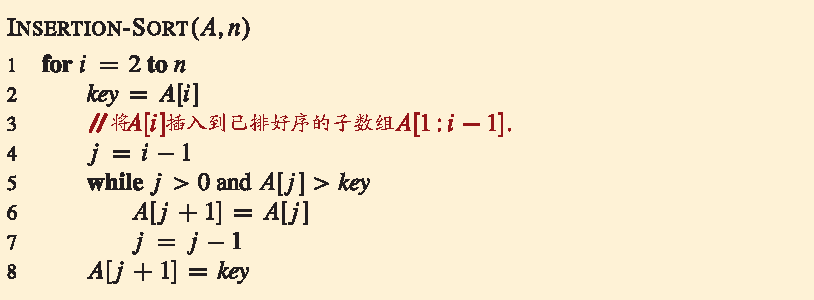
\includegraphics{算法导论第四版插图/第二章/插入排序伪代码.pdf}

我们能观察到伪代码的操作是什么?该过程有嵌套循环。外部循环是一个for循环,无论排序的值如何,它都会运行$n-1$次。内部循环是一个while循环,但它的迭代次数取决于被排序的值。循环变量$j$从$i-1$开始,在每次迭代中递减1,直到它达到0或$A[j]\leq key$。对于给定的$i$值,while循环可能迭代0次,$i-1$次或任何在它们之间。while循环的主体(第6-7行)每次迭代都需要恒定的时间。

这些观察足以推导出INSERTION-SORT的任何情况的$O\left(n^2\right)$运行时间,给我们一个适用于所有输入的总体陈述。运行时间由内部循环主导。因为外部循环的$n-1$次迭代中的每一次都会导致内部循环最多迭代$i-1$次,并且因为$i$最多为$n$,内部循环的总迭代次数最多为$(n-1)(n-1)$,小于$n^2$。由于内部循环的每次迭代都需要恒定的时间,内部循环中花费的总时间最多是常数乘以$n^2$,即$O\left(n^2\right)$。

通过一点创造力,我们还可以看到INSERTION-SORT的最坏情况运行时间是$\Omega\left(n^2\right)$。通过说一个算法的最坏情况运行时间是$\Omega\left(n^2\right)$,我们的意思是对于每个大于某个阈值的输入大小$n$,都存在大小为$n$的至少一个输入,使得该算法需要至少$c n^2$时间,其中$c$是某个正常数。这并不一定意味着算法对于所有输入都需要至少$c n^2$时间。

现在让我们看看为什么INSERTION-SORT的最坏情况运行时间是$\Omega\left(n^2\right)$。对于一个值要移到它起始位置的右侧,它必须在第6行中被移动。实际上,对于一个值要移动到它起始位置的右侧$k$个位置,第6行必须执行$k$次。如图3.1所示,让我们假设$n$是3的倍数,这样我们就可以将数组$A$分成$n/3$个位置的组。假设在INSERTION-SORT的输入中,$n/3$个最大值占据了前$n/3$个数组位置$A[1:n/3]$。(它们在前$n/3$个位置内的相对顺序并不重要。)一旦数组被排序,这$n/3$个值中的每一个都会在最后$n/3$个位置$A[2n/3+1:n]$中的某个位置结束。为了实现这一点,这$n/3$个值中的每一个都必须通过中间的$n/3$个位置$A[n/3+1:2n/3]$。这$n/3$个值中的每一个都会逐个通过这些中间的$n/3$个位置,至少需要通过第6行$n/3$次。因为至少有$n/3$个值必须通过至少$n/3$个位置,所以INSERTION-SORT在最坏情况下所需的时间至少与$(n/3)(n/3)=n^2/9$成正比,即$\Omega\left(n^2\right)$。

因为我们已经证明了INSERTION-SORT在所有情况下都以$O\left(n^2\right)$时间运行,并且存在一种输入使其需要$\Omega\left(n^2\right)$时间,因此我们可以得出结论,INSERTION-SORT的最坏情况运行时间是$\Theta\left(n^2\right)$。上下界的常数因子可能不同并不重要。重要的是我们已经在常数因子(不计低阶项)范围内表征了最坏情况的运行时间。这个论点并没有表明INSERTIONSORT在所有情况下都以$\Theta\left(n^2\right)$时间运行。实际上,我们在第2章中看到,最好情况的运行时间是$\Theta(n)$。

\section{渐进记号:形式化定义}

在非正式地了解渐进符号后,让我们更加正式。我们用来描述算法渐进运行时间的符号是基于函数定义的,这些函数的定义域通常是自然数集合$\mathbb{N}$或实数集合$\mathbb{R}$。这些符号方便描述运行时间函数$T(n)$。本节定义了基本的渐进符号,并介绍了一些常见的“适当”的符号滥用。

\begin{figure}
    \centering
    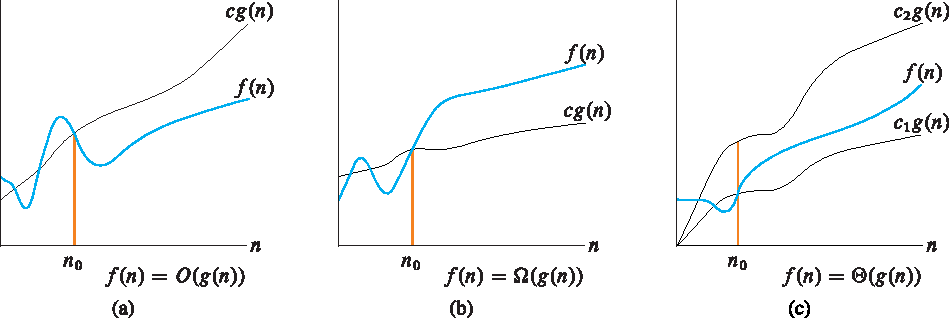
\includegraphics{算法导论第四版插图/第二章/渐进时间复杂度比较示意图.pdf}
    \caption{图是$O, \Omega$和$\Theta$符号的图形示例。在每个部分中,显示的$n_0$值是最小可能值,但任何更大的值也可以。 (a) $O$符号给出函数的上界,精确到一个常数因子。如果存在正常数$n_0$和$c$使得在$n_0$及其右侧,$f(n)$的值总是在或低于$cg(n)$上,则我们写作$f(n)=O(g(n))$。 (b) $\Omega$符号给出函数的下界,精确到一个常数因子。如果存在正常数$n_0$和$c$使得在$n_0$及其右侧,$f(n)$的值总是在或高于$cg(n)$上,则我们写作$f(n)=\Omega(g(n))$。 (c) $\Theta$符号将函数约束在常数因子之内。如果存在正常数$n_0,c_1$和$c_2$使得在$n_0$及其右侧,$f(n)$的值总是在$c_1g(n)$和$c_2g(n)$之间,则我们写作$f(n)=\Theta(g(n))$。}
    \label{渐进时间复杂度比较示意图}
\end{figure}

\textbf{$O$记号}

正如我们在第3.1节中所看到的,$O$符号描述了一个渐进上界。我们使用$O$符号给出一个函数的上界,精确到一个常数因子。
以下是$O$符号的正式定义。对于给定的函数$g(n)$,我们用$O(g(n))$(发音为“big-oh of $g$ of $n$”或有时简称为“oh of $g$ of $n$”)表示函数集合
$O(g(n))=\left\{f(n)\right.$ : 存在正常数$c$和$n_0$,使得
$$
\left.0 \leq f(n) \leq c g(n) \text { for all } n \geq n_0\right\} .{ }^1
$$
如果存在正常数$c$使得$f(n) \leq c g(n)$对于足够大的$n$成立,则函数$f(n)$属于集合$O(g(n))$。图3.2(a)展示了$O$符号的直观理解。对于所有大于等于$n_0$的$n$值,函数$f(n)$的值都在或低于$cg(n)$上。

$O(g(n))$的定义要求集合中的每个函数$f(n)$都是渐进非负的:只要$n$足够大,$f(n)$必须是非负的。(渐进正函数是指对于所有足够大的$n$,函数都是正的。)因此,函数$g(n)$本身必须是渐进非负的,否则集合$O(g(n))$为空。因此,我们假设在$O$符号中使用的每个函数都是渐进非负的。这个假设也适用于本章中定义的其他渐进符号。

您可能会惊讶我们是如何用集合来定义$O$符号的。实际上,您可能会期望我们会写“$f(n) \in O(g(n))$”,以表示$f(n)$属于集合$O(g(n))$。相反,我们通常写“$f(n)=O(g(n))$”,并说“$f(n)$是big-oh of $g(n)$”,以表达相同的概念。虽然一开始可能会感到混乱,但在本节后面我们将看到这样做的好处。

让我们探讨一个例子,说明如何使用$O$符号的正式定义来证明我们丢弃低阶项和忽略最高阶项的常数系数的做法是正确的。我们将展示$4 n^2+100 n+500=O\left(n^2\right)$,即使低阶项的系数比主项大得多。我们需要找到正常数$c$和$n_0$,使得对于所有$n \geq n_0$,都有$4 n^2+100 n+500 \leq c n^2$。将两边都除以$n^2$得到$4+100 / n+500 / n^2 \leq c$。这个不等式对于许多$c$和$n_0$的选择都成立。例如,如果我们选择$n_0=1$,那么这个不等式对于$c=604$成立。如果我们选择$n_0=10$,那么$c=19$可以工作,选择$n_0=100$允许我们使用$c=5.05$。

我们也可以使用$O$符号的正式定义来证明函数$n^3-100 n^2$不属于集合$O\left(n^2\right)$,即使$n^2$的系数是一个大的负数。如果我们有$n^3-100 n^2=O\left(n^2\right)$,那么就会有正常数$c$和$n_0$,使得对于所有$n \geq n_0$,都有$n^3-100 n^2 \leq c n^2$。同样,我们将两边都除以$n^2$,得到$n-100 \leq c$。无论我们为常数$c$选择什么值,这个不等式都不成立,对于任何$n>c+100$的值都不成立。

\textbf{$\Omega$记号}

正如$O$符号提供了一个函数的渐进上界,$\Omega$符号提供了一个渐进下界。对于给定的函数$g(n)$,我们用$\Omega(g(n))$(读作“big-omega of $g$ of $n$”或有时简称“omega of $g$ of $n$”)表示函数集合:
$\Omega(g(n))=\left\{f(n)\right.$:存在正常数$c$和$n_0$,使得对于所有$\left.n \geq n_0\right\}$,都有$0 \leq c g(n) \leq f(n)$。
图3.2(b)展示了$\Omega$符号的直观理解。对于所有$n$值,包括或在$n_0$右侧的值,$f(n)$的值在或以上$c g(n)$。

我们已经展示了$4 n^2+100 n+500=O\left(n^2\right)$。现在让我们展示$4 n^2+100 n+500=\Omega\left(n^2\right)$。我们需要找到正常数$c$和$n_0$,使得对于所有$n \geq n_0$,都有$4 n^2+100 n+500 \geq c n^2$。与之前一样,我们将两边都除以$n^2$,得到$4+100 / n+500 / n^2 \geq c$。当$n_0$为任何正整数且$c=4$时,这个不等式成立。

如果我们从$4n^2$项中减去低阶项而不是加上它们会怎么样?如果$n^2$项的系数很小怎么办?函数仍然是$\Omega\left(n^2\right)$。例如,让我们展示$n^2 / 100-100 n-500=\Omega\left(n^2\right)$。除以$n^2$得到$1 / 100-100 / n-500 / n^2 \geq c$。我们可以选择任何大于或等于10,005的$n_0$值,并找到一个正值$c$。例如,当$n_0=10,005$时,我们可以选择$c=2.49 \times 10^{-9}$。是的,那是一个非常小的$c$值,但它是正数。如果我们选择更大的$n_0$值,我们也可以增加$c$值。例如,如果$n_0=100,000$,那么我们可以选择$c=0.0089$。$n_0$值越高,我们就越可以选择接近系数$1 / 100$的$c$值。

\textbf{$\Theta$记号}

我们使用$\Theta$符号表示渐进紧密界限。对于给定的函数$g(n)$,我们用$\Theta(g(n))$(读作“theta of $g$ of $n$”)表示函数集合:
$\Theta(g(n))=\left\{f(n)\right.$:存在正常数$c_1, c_2$和$n_0$,使得对于所有$\left.n \geq n_0\right\}$,都有$0 \leq c_1 g(n) \leq f(n) \leq c_2 g(n)$。
图3.2(c)展示了$\Theta$符号的直观理解。对于所有$n$值,包括或在$n_0$右侧的值,$f(n)$的值在或以上$c_1 g(n)$并在或以下$c_2 g(n)$。换句话说,对于所有$n \geq n_0$,函数$f(n)$与常数因子内的$g(n)$相等。

$O-, \Omega-$和$\Theta$符号的定义导致以下定理,其证明我们留作练习3.2-4。

\begin{theorem}{}{定理3.1}
对于任何两个函数$f(n)$和$g(n)$,当且仅当$f(n)=O(g(n))$且$f(n)=\Omega(g(n))$时,我们有$f(n)=\Theta(g(n))$。
\end{theorem}

我们一般将定理\ref{thm:定理3.1}用在证明渐进紧界上面,也就是用渐进上界和渐进下界来证明渐进紧界。

\textbf{渐进记号和运行时间}

当使用渐进符号来描述算法的运行时间时,确保所使用的渐进符号尽可能精确,而不会过度陈述其适用于哪个运行时间。以下是一些使用渐进符号来描述运行时间的正确和不正确的示例。

让我们从插入排序开始。我们可以正确地说插入排序的最坏运行时间是$O\left(n^2\right), \Omega\left(n^2\right)$,并且由于\ref{thm:定理3.1},$\Theta\left(n^2\right)$。虽然三种描述最坏情况运行时间的方式都是正确的,但$\Theta\left(n^2\right)$界限是最精确和最受欢迎的。同样地,我们可以正确地说插入排序的最佳情况运行时间为$O(n), \Omega(n)$和$\Theta(n)$,其中$\Theta(n)$最精确,因此最受欢迎。

以下是我们不能正确说的内容:插入排序的运行时间是$\Theta\left(n^2\right)$。这是一种夸大其词的说法,因为通过省略声明中的“最坏情况”,我们留下了一个涵盖所有情况的概括性陈述。错误在于插入排序并不总是在$\Theta\left(n^2\right)$时间内运行,因为正如我们所见,它在最佳情况下运行时间为$\Theta(n)$。但我们可以正确地说插入排序的运行时间是$O\left(n^2\right)$,因为在所有情况下,它的运行时间都不会超过$n^2$。当我们使用$O\left(n^2\right)$而不是$\Theta\left(n^2\right)$时,没有问题出现,即使有些情况下运行时间增长得比$n^2$慢。同样地,我们不能正确地说插入排序的运行时间是$\Theta(n)$,但我们可以说它的运行时间是$\Omega(n)$。

归并排序呢?由于归并排序在所有情况下都以$\Theta(n\lg n)$时间运行,我们可以只说它的运行时间是$\Theta(n\lg n)$,而不指定最坏情况、最佳情况或任何其他情况。

有时人们会混淆$O$符号和$\Theta$符号,错误地使用$O$符号来表示渐进紧密界限。他们会说:“一个$O(n\lg n)$时间复杂度的算法比一个$O\left(n^2\right)$时间复杂度的算法运行得更快。”也许是这样,也许不是。由于$O$符号仅表示渐进上界,所谓的$O\left(n^2\right)$时间复杂度的算法实际上可能在$\Theta(n)$时间内运行。您应该小心选择适当的渐进符号。如果要表示渐进紧密界限,请使用$\Theta$符号。

我们通常使用渐进符号来提供最简单和最精确的界限。例如,如果一个算法在所有情况下的运行时间为$3n^2+20n$,我们使用渐进符号来写出它的运行时间为$\Theta\left(n^2\right)$。严格来说,我们也可以写出运行时间为$O\left(n^3\right)$或$\Theta\left(3n^2+20n\right)$。然而,在这种情况下,这些表达式都不如写$\Theta\left(n^2\right)$有用:如果运行时间为$3n^2+20n$,那么$O\left(n^3\right)$不如$\Theta\left(n^2\right)$精确,而$\Theta\left(3n^2+20n\right)$引入了复杂性,混淆了增长的顺序。通过编写最简单和最精确的界限,例如$\Theta\left(n^2\right)$,我们可以对不同的算法进行分类和比较。在整本书中,您将看到几乎所有的渐进运行时间都基于多项式和对数函数:例如$n,n \lg ^2 n,n^2 \lg n$或$n^{1 / 2}$。您还将看到其他一些函数,例如指数、$\lg \lg n$和$\lg ^* n$(请参见第3.3节)。通常很容易比较这些函数的增长速度。问题3-3会给您提供良好的练习。

\textbf{等式和不等式中的渐进记号}

虽然我们正式地将渐进符号定义为集合,但在公式中,我们使用等号$(=)$而不是集合成员符号$(\in)$。例如,我们写道$4n^2+100n+500=O\left(n^2\right)$。我们还可以写成$2n^2+3n+1=2n^2+\Theta(n)$。我们如何解释这样的公式?

当渐进符号单独出现在等式(或不等式)的右侧时,例如$4n^2+100n+500=O\left(n^2\right)$,等号表示集合成员关系:$4n^2+100n+500 \in O\left(n^2\right)$。然而,通常情况下,当渐进符号出现在公式中时,我们将其解释为代表某个我们不想命名的匿名函数。例如,公式$2n^2+3n+1=2n^2+\Theta(n)$表示$2n^2+3n+1=2n^2+f(n)$,其中$f(n) \in \Theta(n)$。在这种情况下,我们让$f(n)=3n+1$,它确实属于$\Theta(n)$。

以这种方式使用渐进符号可以帮助消除方程中不必要的细节和杂乱。例如,在第2章中,我们将归并排序的最坏运行时间表示为递归式
$$
T(n)=2 T(n / 2)+\Theta(n)
$$
如果我们只关心$T(n)$的渐进行为,那么没有必要准确指定所有低阶项,因为它们都被理解为包含在由术语$\Theta(n)$表示的匿名函数中。

\textbf{渐进记号的适当的滥用}

\textbf{$o$记号}

\textbf{$\omega$记号}

\textbf{比较函数}

\textbf{传递性}

\textbf{反身性}

\textbf{对称性}



\section{标准记号和常用函数}

\chapter{分治策略}

\section{矩阵相乘}

\section{矩阵相乘的Strassen算法}

\section{用代入法求解递归式}

\section{用递归树方法求解递归式}

\section{用主方法求解递归式}

\chapter{概率分析与随机算法}

\section{雇佣问题}

\section{指示器随机变量}

\section{随机算法}

\section{概率分析和指示器随机变量的进一步使用}

\part{排序和顺序统计量}

\chapter*{简介}

\chapter{堆排序}

\chapter{快速排序}

\chapter{线性时间排序}

\chapter{中位数和顺序统计量}

\part{数据结构}

\chapter*{简介}

\chapter{基本数据结构}

\chapter{哈希表}

\chapter{二叉搜索树}

\chapter{红黑树}

\part{高级设计与分析技术}

\chapter*{简介}

\chapter{动态规划}

\chapter{贪心算法}

\chapter{均摊分析}

\part{高级数据结构}

\chapter*{简介}

\chapter{增强数据结构}

\chapter{B树}

\chapter{用于不相交集合的数据结构}

\part{图算法}

\chapter*{简介}

\chapter{基本的图算法}

\chapter{最小生成树}

\chapter{单源最短路径}

\chapter{所有结点对的最短路径问题}

\chapter{最大流}

\chapter{二部图匹配}

\part{算法问题选编}

\chapter*{简介}

\chapter{并行算法}

\chapter{在线算法}

\chapter{矩阵操作}

\chapter{线性规划}

\chapter{多项式与快速傅立叶变换}

\chapter{数论算法}

\chapter{字符串匹配}

\chapter{机器学习算法}

\chapter{NP完全性}

\chapter{近似算法}

\part{附录:数学基础知识}

\chapter*{简介}

\chapter*{求和}

\chapter*{集合}

\chapter*{计数和概率}

\chapter*{矩阵}

\end{document}